% ============================================================
% Charla para colegas de CEAZA (español) --- reconstrucción de gaps
% en series ambientales costeras, caso Tongoy (clorofila-a y oxígeno).
%
% NO es una traducción de manuscript/presentation/main.tex (charla de
% pasantía, en inglés). Es una charla nueva, más larga, pensada para
% oceanógrafos/meteorólogos/técnicos de monitoreo, terminando en una
% demostración práctica en vivo (ver demo/).
%
% Compila con Tectonic desde esta carpeta:
%   tectonic main.tex
%
% Estilo y macros (\statcard, \takeaway, \caution, \cmpbox, \yes/\weak/\no)
% adaptados del preámbulo de manuscript/presentation/main.tex -- ese
% archivo original NO fue modificado.
% ============================================================
\documentclass[aspectratio=169,11pt]{beamer}

\usepackage[utf8]{inputenc}
\usepackage[T1]{fontenc}
\usepackage{lmodern}
\usefonttheme{serif}
\usepackage{amsmath,amssymb}
\usepackage{booktabs}
\usepackage{array}
\usepackage{graphicx}
\usepackage{adjustbox}
\usepackage{xcolor}
\usepackage{tikz}
\usetikzlibrary{arrows.meta,positioning,decorations.pathreplacing,calc,fit}
\usepackage{appendixnumberbeamer}

\setbeamertemplate{navigation symbols}{}
\beamertemplatenavigationsymbolsempty

% ── Paleta (misma que la charla en inglés, para consistencia visual) ──
\definecolor{ink}{HTML}{2B2B2B}
\definecolor{accent}{HTML}{1E6E7A}
\definecolor{accentlt}{HTML}{2A7F8E}
\definecolor{tsviolet}{HTML}{5E4B9B}
\definecolor{slate}{HTML}{5F7F8A}
\definecolor{cgreen}{HTML}{1B9E77}
\definecolor{cblue}{HTML}{3B6FA0}
\definecolor{camber}{HTML}{C0791F}
\definecolor{cred}{HTML}{B24743}
\definecolor{faint}{HTML}{8A9299}
\definecolor{panel}{HTML}{F4F6F7}

\setbeamercolor{normal text}{fg=ink}
\setbeamercolor{frametitle}{fg=accent}
\setbeamercolor{structure}{fg=accent}
\setbeamercolor{itemize item}{fg=accent}
\setbeamercolor{itemize subitem}{fg=accentlt}

\setbeamerfont{frametitle}{size=\Large,series=\bfseries,family=\sffamily}
\setbeamerfont{title}{size=\LARGE,series=\bfseries,family=\sffamily}

\setbeamertemplate{itemize item}{\small\color{accent}\ensuremath{\bullet}}
\setbeamertemplate{itemize subitem}{\scriptsize\color{accentlt}\ensuremath{\circ}}
\setbeamertemplate{enumerate item}{\color{accent}\insertenumlabel.}

\setbeamertemplate{frametitle}{%
  \nointerlineskip
  \vskip0.85em
  \hbox to\paperwidth{\hskip0.75cm
    \vtop{\hsize=\dimexpr\paperwidth-1.5cm\relax\raggedright
      {\usebeamerfont{frametitle}\usebeamercolor[fg]{frametitle}\insertframetitle\par}%
      \vskip3pt{\color{accent}\hrule height1pt}%
    }\hskip0.75cm}%
  \vskip2pt
}

\setbeamertemplate{footline}{%
  \vskip3pt
  {\color{faint!45}\hrule height0.4pt width\paperwidth}
  \vskip3pt
  \hbox to\paperwidth{\hskip0.75cm
    {\scriptsize\color{faint}Reconstrucción de gaps en series costeras}%
    \hfil{\scriptsize\color{faint}Matteo Faverio\;\textperiodcentered\;CEAZA}\hfil
    {\scriptsize\color{faint}\insertframenumber}\hskip0.75cm}%
  \vskip4pt
}

\newcommand{\chl}{Cl\,\textit{a}}

\newcommand{\statcard}[3]{%
  \begin{tikzpicture}
    \node[rounded corners=3pt,draw=#1,line width=0.9pt,fill=#1!7,inner sep=0pt,
          minimum width=2.95cm]
      {\begin{minipage}[c][1.85cm][c]{2.95cm}\centering
         {\large\bfseries\color{#1}#2}\par\vskip5pt{\scriptsize\color{ink}#3}
       \end{minipage}};
  \end{tikzpicture}%
}
\newcommand{\takeaway}[1]{%
  \par\vspace{3pt}\noindent
  \begin{tikzpicture}
    \node[rounded corners=2pt,draw=accent!55,line width=0.7pt,fill=accent!10,inner sep=7pt]
      {\parbox{\dimexpr\linewidth-22pt\relax}{\raggedright\color{ink}#1}};
  \end{tikzpicture}\par
}
\newcommand{\caution}[1]{%
  \par\vspace{3pt}\noindent
  \begin{tikzpicture}
    \node[rounded corners=2pt,draw=cred!55,line width=0.7pt,fill=cred!8,inner sep=7pt]
      {\parbox{\dimexpr\linewidth-22pt\relax}{\raggedright\color{ink}#1}};
  \end{tikzpicture}\par
}
\newcommand{\cmpbox}[3]{%
  \begin{tikzpicture}
    \node[rounded corners=3pt,draw=#1,line width=1pt,fill=#1!7,inner sep=7pt]
      {\parbox{#2}{\raggedright\color{ink}#3}};
  \end{tikzpicture}%
}
\newcommand{\srcline}[1]{\vfill\hbox to\linewidth{{\tiny\color{faint}#1}\hfil}}

\newcommand{\yes}{\textcolor{cgreen}{\textbf{\checkmark}}}
\newcommand{\weak}{\textcolor{camber}{\textbf{\raisebox{0.1ex}{$\sim$}}}}
\newcommand{\no}{\textcolor{cred}{\textbf{$\times$}}}

\title{Reconstrucción de gaps en series ambientales costeras}
\author{Matteo Faverio}
\date{2026}

\begin{document}

% ───────────────────────── DIAPOSITIVA 1: TÍTULO ──────────────────
{\setbeamertemplate{footline}{}
\begin{frame}[plain]
  \vskip0.6cm
  \hbox to\paperwidth{\hskip1.1cm\vtop{\hsize=\dimexpr\paperwidth-2.2cm\relax\raggedright
    {\color{accent}\rule{2.6cm}{2.2pt}}\par\vskip0.5cm
    {\sffamily\bfseries\fontsize{21}{25}\selectfont\color{ink}
      Reconstrucción de gaps en\\ series ambientales costeras\par}
    \vskip0.30cm
    {\sffamily\large\color{accentlt}Un flujo de trabajo reutilizable, con el caso de Tongoy\\
      (clorofila-\textit{a} y oxígeno disuelto) como ejemplo\par}
    \vskip0.55cm
    {\color{faint}\rule{\linewidth}{0.5pt}}\par\vskip0.32cm
    {\sffamily\large\color{ink}\textbf{Matteo Faverio}\par}
    \vskip0.08cm
    {\sffamily\footnotesize\color{faint}CEAZA --- Centro de Estudios Avanzados en Zonas \'Aridas\par}
    \vskip0.03cm
    {\sffamily\footnotesize\color{faint}Charla para colegas \;\textperiodcentered\; 2026\par}
  }\hskip1.1cm}
  \vfill
  \hbox to\paperwidth{\hskip1.1cm\parbox{\dimexpr\paperwidth-2.2cm\relax}{%
    {\footnotesize\color{accent}Objetivo de hoy:} {\footnotesize\color{faint}entender cómo se
     reconstruye un gap de forma validada, ver TS-ICL corriendo en vivo, y dejarlos con un
     ejemplo que puedan correr en su propia serie.}}\hfil}
  \vskip0.55cm
\end{frame}}

% ═══════════════ BLOQUE A --- EL PROBLEMA OPERATIVO ═══════════════

% ───────────────────────── DIAPOSITIVA 2 ──────────────────────────
\begin{frame}[t]{Los registros in situ se interrumpen}
  \vskip4pt
  \begin{center}
    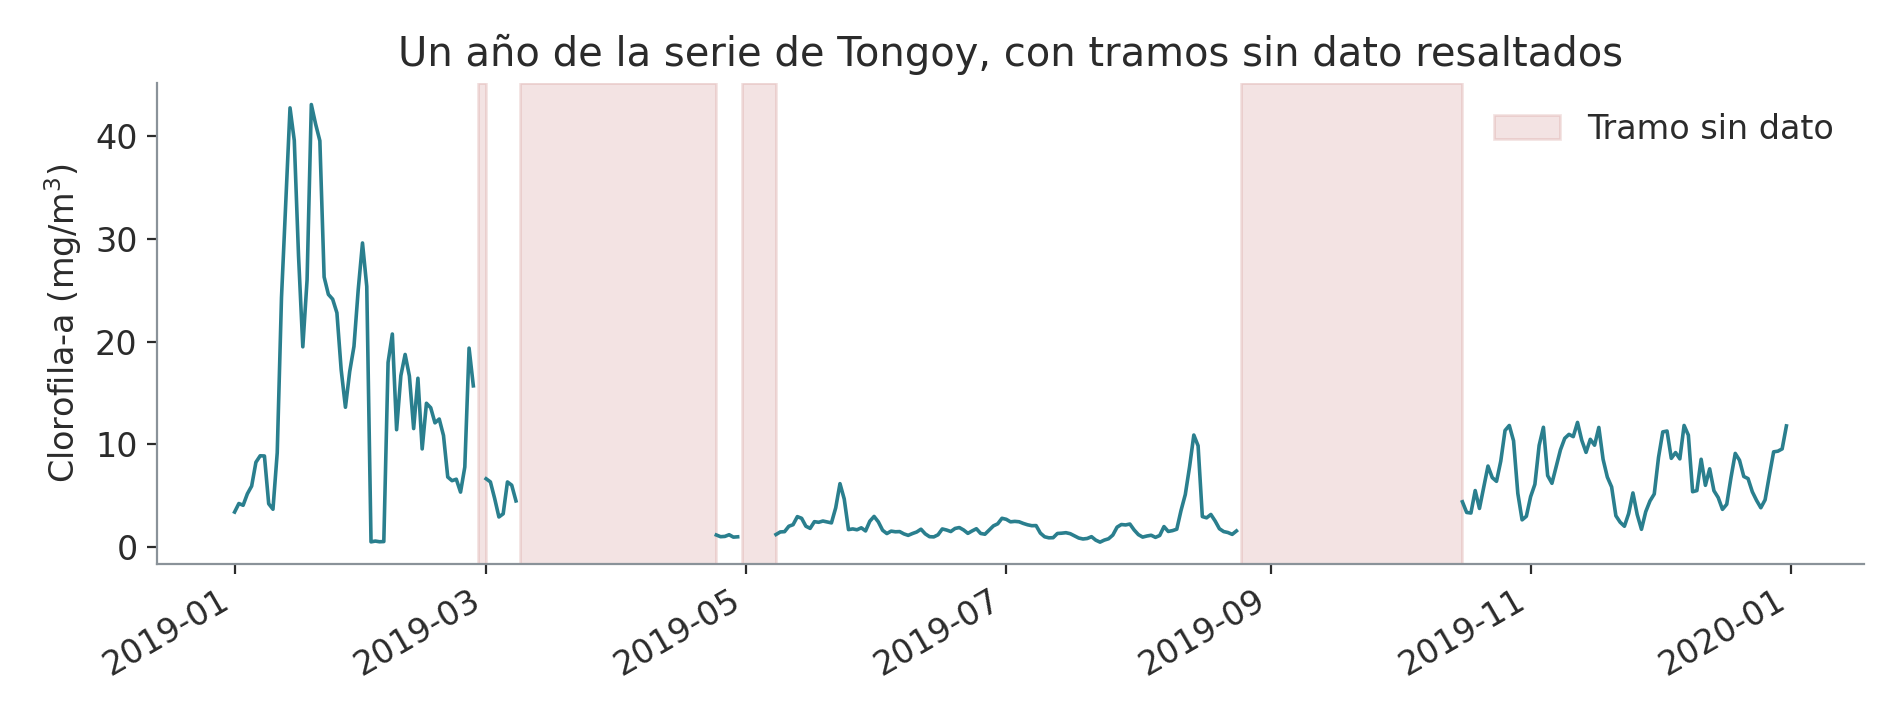
\includegraphics[width=0.92\textwidth]{figures/fig_a_gap_example.png}
  \end{center}
  \vskip4pt
  {\footnotesize\color{ink}Mantenimiento, biofouling, fallas de comunicación, calibración.
   Un año cualquiera de la boya de Tongoy ya muestra el problema: reconstruir gaps no es
   opcional si se quiere usar la serie completa.}
\end{frame}

% ───────────────────────── DIAPOSITIVA 3 ──────────────────────────
\begin{frame}[t]{Reconstrucción retrospectiva de gaps cerrados}
  \vskip8pt
  \begin{columns}[T]
    \begin{column}{0.55\textwidth}
      {\small
      \begin{itemize}\setlength\itemsep{0.22cm}
        \item Reconstruir un gap ya cerrado es distinto de predecir el futuro.
        \item Varios métodos usan datos observados \textbf{antes y después} del gap como
          contexto de reconstrucción.
        \item Eso es válido para un gap cerrado, pero esos mismos métodos no son
          directamente aplicables a un gap abierto, sin datos posteriores todavía.
      \end{itemize}}
    \end{column}
    \begin{column}{0.42\textwidth}
      \cmpbox{accent}{\linewidth}{\centering
        {\scriptsize\color{ink}...observado\; \textbf{[ ? ? ? ]}\; observado...}\\[6pt]
        {\footnotesize\color{accent}$\uparrow$\hspace{2.1cm}$\uparrow$}\\
        {\scriptsize contexto antes\hspace{0.6cm}contexto después}}
    \end{column}
  \end{columns}
  \vskip0.25cm
  \takeaway{\footnotesize Hoy hablamos, sobre todo, de \textbf{reconstrucción
   retrospectiva}. Qué método sirve para un gap abierto se retoma en la diapositiva de
   capacidades más adelante.}
\end{frame}

% ───────────────────────── DIAPOSITIVA 4 ──────────────────────────
\begin{frame}[t]{El sitio y los datos: boya de Tongoy}
  \vskip4pt
  \begin{center}
    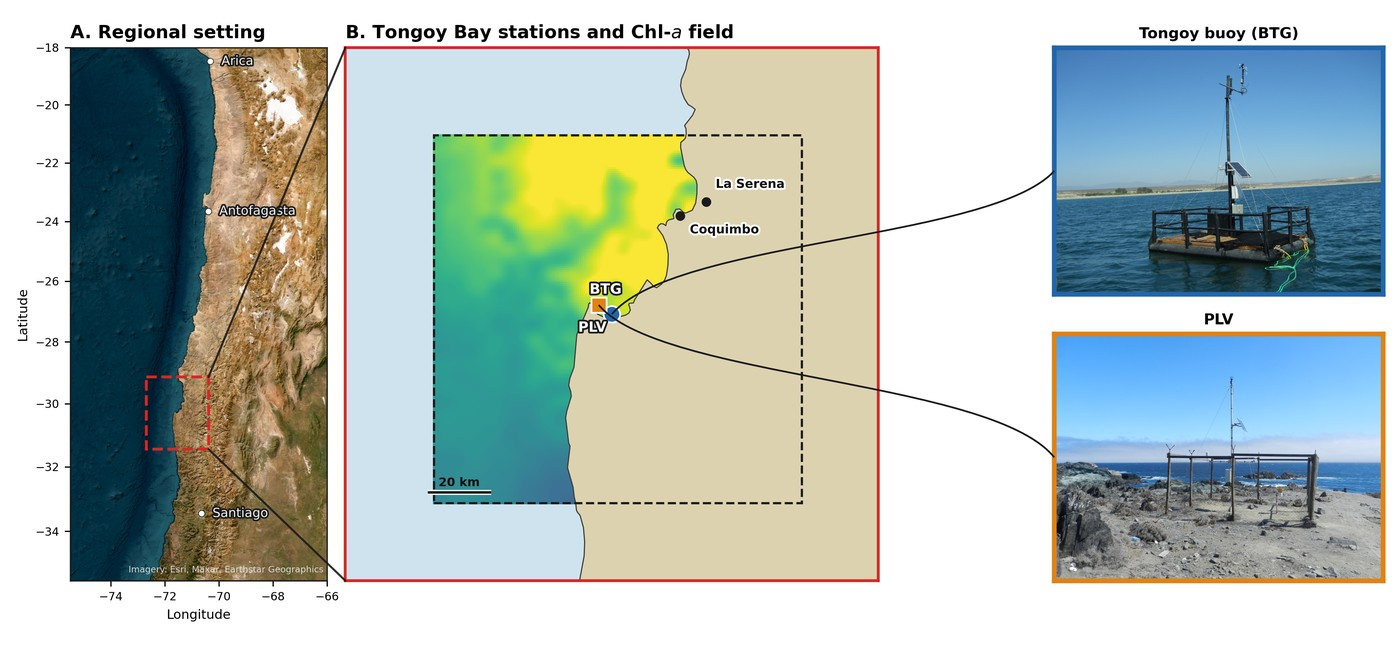
\includegraphics[width=0.62\textwidth,trim=0 6 0 6,clip]{figures/fig1_site_context.jpg}
  \end{center}
  \vskip6pt
  \begin{center}\footnotesize
  \begin{tabular}{@{}ll@{}}
    \toprule
    Variable & Rol en esta charla\\
    \midrule
    Clorofila-\textit{a} in situ (BTGCLF) & objetivo principal, caso 1\\
    Oxígeno disuelto in situ (BTGOXD2) & objetivo, caso 2\\
    Viento y surgencia costera (PLV) & covariable física\\
    Clorofila satelital, temperatura superficial & covariable de producto externo\\
    \bottomrule
  \end{tabular}
  \end{center}
\end{frame}

% ───────────────────────── DIAPOSITIVA 5 ──────────────────────────
\begin{frame}[t]{Por qué el problema no es trivial}
  \vskip6pt
  \begin{columns}[T]
    \begin{column}{0.45\textwidth}
      \vskip0.35cm
      \centering
      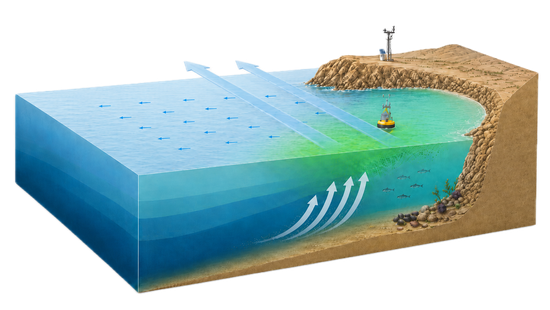
\includegraphics[width=0.92\linewidth]{figures/fig_upwelling_schematic.png}
      \vskip0.10cm
      {\scriptsize\color{ink}Transporte por viento y surgencia costera cerca de Tongoy.}\\[1pt]
      {\scriptsize\color{faint}Montecino \& Lange (2009).}
    \end{column}
    \begin{column}{0.53\textwidth}
      \vskip0.35cm
      \centering
      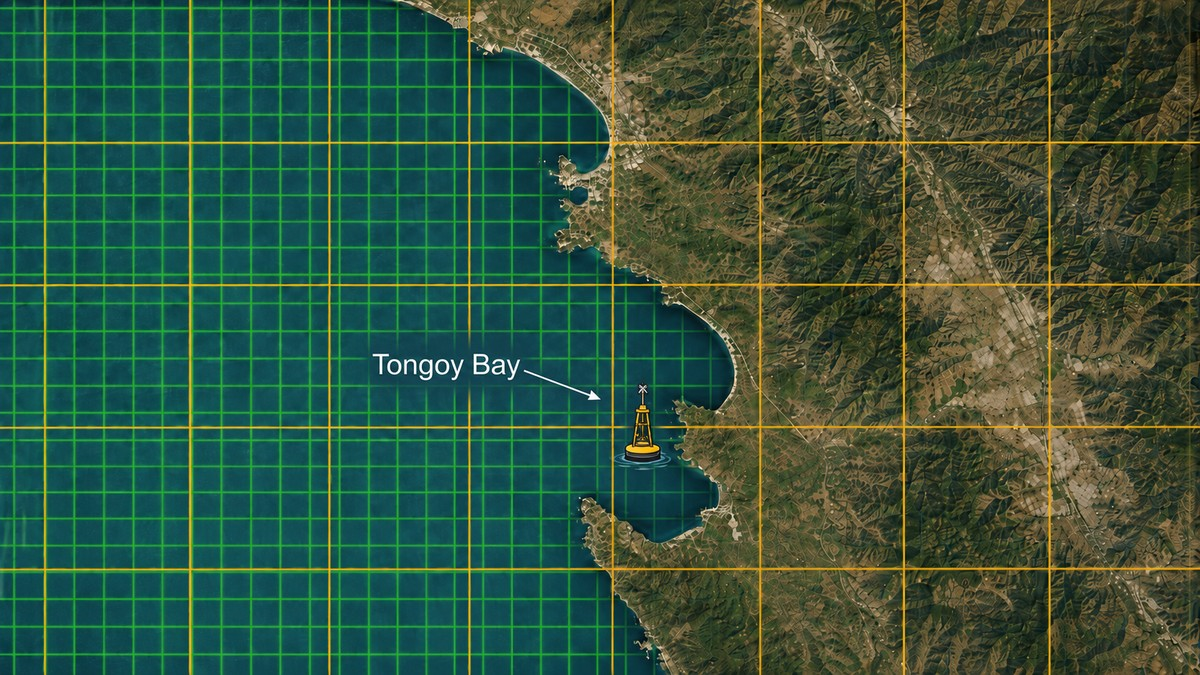
\includegraphics[width=\linewidth]{figures/map.jpg}
    \end{column}
  \end{columns}
  \vskip8pt
  {\footnotesize\color{ink}La boya mide un punto costero. Los productos satelitales y de
   reanálisis son campos de grilla más gruesa: útiles como contexto, pero no observan
   exactamente lo mismo que el sensor local.}
\end{frame}

% ───────────────────────── DIAPOSITIVA 6 ──────────────────────────
\begin{frame}[t]{Qué le pedimos a un método de reconstrucción}
  \vskip10pt
  {\small
  \begin{itemize}\setlength\itemsep{0.28cm}
    \item Reconstruir valores faltantes de forma \textbf{creíble}.
    \item Funcionar también sobre \textbf{gaps reales}.
    \item Poder usar \textbf{covariables} cuando aportan, sin depender de ellas.
    \item Entregar, si es posible, una noción de \textbf{incertidumbre}.
    \item Ser \textbf{operable}: alguien del equipo lo puede correr de nuevo el año que viene.
  \end{itemize}}
  \vskip0.4cm
  \takeaway{Ningún método cumple los cinco puntos igual de bien. Por eso se necesita un
   protocolo de comparación, no una elección a priori.}
\end{frame}

% ═══════════════ BLOQUE B --- EL FLUJO Y LA VALIDACIÓN ═══════════════

% ───────────────────────── DIAPOSITIVA 7: PIPELINE ────────────────
\begin{frame}[t]{El flujo de trabajo, de punta a punta}
  \vskip6pt
  \begin{center}
  \resizebox{0.98\textwidth}{!}{%
  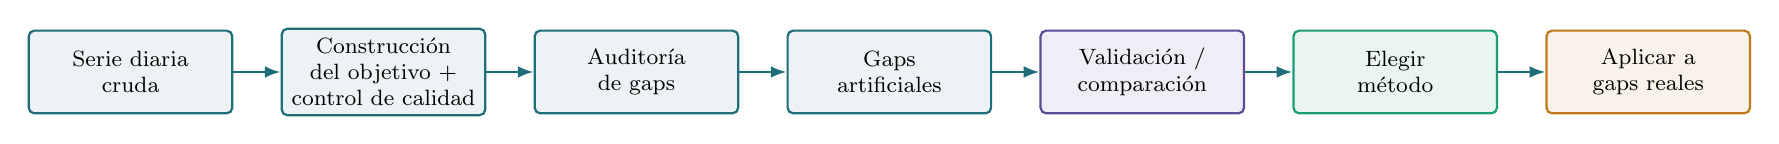
\begin{tikzpicture}[
      node distance=6mm,
      box/.style={rounded corners=2pt, draw=accent, fill=accent!8, line width=0.8pt,
                   minimum height=1.05cm, text width=2.35cm, align=center, font=\footnotesize},
      arr/.style={-{Latex[length=2mm]}, accent, line width=0.9pt}
    ]
    \node[box] (a) {Serie diaria\\cruda};
    \node[box, right=of a] (b) {Construcción\\del objetivo + control de calidad};
    \node[box, right=of b] (c) {Auditoría\\de gaps};
    \node[box, right=of c] (d) {Gaps\\artificiales};
    \node[box, right=of d, fill=tsviolet!10, draw=tsviolet] (e) {Validación /\\comparación};
    \node[box, right=of e, fill=cgreen!10, draw=cgreen] (f) {Elegir\\método};
    \node[box, right=of f, fill=camber!10, draw=camber] (g) {Aplicar a\\gaps reales};
    \draw[arr] (a) -- (b); \draw[arr] (b) -- (c); \draw[arr] (c) -- (d);
    \draw[arr] (d) -- (e); \draw[arr] (e) -- (f); \draw[arr] (f) -- (g);
  \end{tikzpicture}}
  \end{center}
  \vskip0.5cm
  {\footnotesize\color{ink}Este es el mismo flujo para clorofila y para oxígeno, y es el mismo
   flujo que se propone reusar sobre otra variable u otra estación CEAZA. Lo que cambia entre
   series es el resultado de la validación, no la secuencia de pasos.}
\end{frame}

% ───────────────────────── DIAPOSITIVA 8 ──────────────────────────
\begin{frame}[t]{Cómo validamos sin engañarnos}
  \vskip4pt
  \begin{columns}[T]
    \begin{column}{0.60\textwidth}
      \vskip0.15cm
      {\small
      \textbf{Gap artificial.} Escondemos un tramo que sí conocemos, reconstruimos, y
      comparamos contra el valor real.\par\vskip0.25cm
      \textbf{Gap real.} Reconstruimos valores que nunca se observaron --- no hay cómo
      calcular un error.}
    \end{column}
    \begin{column}{0.38\textwidth}
      \caution{\centering Un gap real reconstruido es un \textbf{resultado}, no evidencia
       de validación.}
    \end{column}
  \end{columns}
  \vskip0.35cm
  \begin{center}
    \resizebox{0.98\textwidth}{!}{% Copia traducida (ES) de manuscript/presentation/figures/fig3_validation_schematic_tikz.tex.
% El original en ingles no se modifica. Misma logica de dibujo, solo cambian las etiquetas.
\definecolor{vgObserved}{HTML}{2A7F8E}
\definecolor{vgHidden}{HTML}{C0504D}
\definecolor{vgRecon}{HTML}{1B9E77}
\definecolor{vgMiss}{HTML}{9AA6B2}
\definecolor{vgInk}{HTML}{2B2B2B}

\begin{tikzpicture}[x=0.5cm, y=0.5cm, font=\small,
    obs/.style={fill=vgObserved, draw=vgInk, line width=0.2pt},
    mask/.style={fill=vgHidden, draw=vgInk, line width=0.2pt},
    flow/.style={-{Latex[length=2.1mm]}, vgInk, line width=0.7pt},
    recon/.style={vgRecon, line width=1.3pt, dash pattern=on 3pt off 2pt},
    rdot/.style={circle, fill=vgRecon, draw=none, inner sep=1.0pt}]

  \def\XA{0}   \def\XB{13}  \def\XC{25.4}
  \def\YA{3.4} \def\YB{0.0}

  \node[font=\bfseries, text=vgInk] at (4.9,5.75)  {Serie registrada};
  \node[font=\bfseries, text=vgInk] at (17.9,5.75) {Operación de reconstrucción};
  \node[font=\bfseries, text=vgInk, anchor=west] at (24.6,5.75) {Significado};

  \node[font=\bfseries, text=vgInk, align=center] at (-2.1,3.75) {Gap\\artificial};
  \node[font=\bfseries, text=vgInk, align=center] at (-2.1,0.35) {Gap\\real};

  \draw[vgMiss, line width=0.3pt] (-3.4,1.95) -- (33.6,1.95);

  % ROW 1 -- GAP ARTIFICIAL
  \foreach \i in {0,...,9}{ \fill[obs] (\XA+\i,\YA) rectangle (\XA+\i+0.8,\YA+0.7); }
  \draw[vgHidden, line width=0.7pt, dash pattern=on 2pt off 1.5pt]
      (\XA+3.9,\YA-0.12) rectangle (\XA+6.9,\YA+0.82);
  \draw[decorate,decoration={brace,amplitude=3pt},line width=0.4pt,vgInk]
      (\XA+3.9,\YA+0.95) -- (\XA+6.9,\YA+0.95)
      node[midway,above=1pt,font=\footnotesize,text=vgInk] {valores conocidos};
  \node[font=\small, text=vgInk] at (4.9,\YA-0.75) {valores observados};

  \foreach \i in {0,1,2,3,7,8,9}{ \fill[obs]  (\XB+\i,\YA) rectangle (\XB+\i+0.8,\YA+0.7); }
  \foreach \i in {4,5,6}{        \fill[mask] (\XB+\i,\YA) rectangle (\XB+\i+0.8,\YA+0.7); }
  \draw[recon] plot[smooth] coordinates
      {(\XB+3.9,\YA+0.35) (\XB+4.4,\YA+0.58) (\XB+5.4,\YA+0.18)
       (\XB+6.4,\YA+0.55) (\XB+6.9,\YA+0.33)};
  \foreach \x/\y in {4.4/0.58, 5.4/0.18, 6.4/0.55}{ \node[rdot] at (\XB+\x,\YA+\y) {}; }
  \node[font=\footnotesize, text=vgHidden] at (\XB+5.0,\YA+1.15) {ocultar tramo conocido};
  \node[font=\footnotesize, text=vgRecon]  at (\XB+5.0,\YA-0.55) {reconstruir};

  \node[anchor=west, align=left, text=vgInk] at (\XC-0.25,\YA+0.35)
      {comparar reconstrucción con\\ el valor observado oculto\\
       $\Rightarrow$ calcular error};

  % ROW 2 -- GAP REAL
  \foreach \i in {0,1,2,3,7,8,9}{ \fill[obs] (\XA+\i,\YB) rectangle (\XA+\i+0.8,\YB+0.7); }
  \foreach \i in {4,5,6}{
      \draw[draw=vgMiss,line width=0.4pt] (\XA+\i,\YB) rectangle (\XA+\i+0.8,\YB+0.7);
      \draw[vgMiss,line width=0.4pt] (\XA+\i,\YB)      -- (\XA+\i+0.8,\YB+0.7);
      \draw[vgMiss,line width=0.4pt] (\XA+\i+0.4,\YB)  -- (\XA+\i+0.8,\YB+0.35);
      \draw[vgMiss,line width=0.4pt] (\XA+\i,\YB+0.35) -- (\XA+\i+0.4,\YB+0.7);
  }
  \node[font=\small, text=vgInk] at (4.9,\YB-0.75) {tramo realmente faltante};

  \foreach \i in {0,1,2,3,7,8,9}{ \fill[obs] (\XB+\i,\YB) rectangle (\XB+\i+0.8,\YB+0.7); }
  \foreach \i in {4,5,6}{
      \draw[draw=vgMiss,line width=0.4pt] (\XB+\i,\YB) rectangle (\XB+\i+0.8,\YB+0.7);
      \draw[vgMiss,line width=0.4pt] (\XB+\i,\YB)      -- (\XB+\i+0.8,\YB+0.7);
      \draw[vgMiss,line width=0.4pt] (\XB+\i+0.4,\YB)  -- (\XB+\i+0.8,\YB+0.35);
      \draw[vgMiss,line width=0.4pt] (\XB+\i,\YB+0.35) -- (\XB+\i+0.4,\YB+0.7);
  }
  \draw[recon] plot[smooth] coordinates
      {(\XB+3.9,\YB+0.35) (\XB+4.4,\YB+0.58) (\XB+5.4,\YB+0.18)
       (\XB+6.4,\YB+0.55) (\XB+6.9,\YB+0.33)};
  \foreach \x/\y in {4.4/0.58, 5.4/0.18, 6.4/0.55}{ \node[rdot] at (\XB+\x,\YB+\y) {}; }
  \node[font=\footnotesize, text=vgRecon] at (\XB+5.0,\YB-0.55) {reconstruir};

  \node[anchor=west, align=left, text=vgInk] at (\XC-0.25,\YB+0.35)
      {no hay nada contra que comparar\\
       $\Rightarrow$ no es evidencia de validación};

  \draw[flow] (10.2,\YA+0.35) -- (12.7,\YA+0.35);
  \draw[flow] (10.2,\YB+0.35) -- (12.7,\YB+0.35);
  \draw[flow] (23.1,\YA+0.35) -- (24.7,\YA+0.35);
  \draw[flow] (23.1,\YB+0.35) -- (24.7,\YB+0.35);

\end{tikzpicture}
}
  \end{center}
  \vfill
  \hbox to\linewidth{{\footnotesize\color{accent}Los métodos se ordenan \emph{solo} con gaps
    artificiales --- para clorofila y para oxígeno por igual.}\hfil}
\end{frame}

% ───────────────────────── DIAPOSITIVA 9 ──────────────────────────
\begin{frame}[t]{Por qué no alcanza con separar filas al azar}
  \vskip10pt
  \begin{columns}[T]
    \begin{column}{0.52\textwidth}
      {\small
      \begin{itemize}\setlength\itemsep{0.22cm}
        \item Una serie temporal tiene memoria: el día $t$ se parece al día $t{-}1$.
        \item Separar filas al azar deja, casi siempre, un vecino inmediato del gap
          adentro del conjunto de entrenamiento.
        \item Eso filtra información del propio gap hacia el modelo: el método
          parece mejor de lo que realmente es.
      \end{itemize}}
    \end{column}
    \begin{column}{0.44\textwidth}
      \cmpbox{cred}{\linewidth}{\footnotesize\centering
        \textbf{Split al azar}\\[2pt] filas vecinas al gap pueden quedar en ambos lados
        $\Rightarrow$ fuga de información}
      \vskip8pt
      \cmpbox{cgreen}{\linewidth}{\footnotesize\centering
        \textbf{Bloques temporales}\\[2pt] el gap completo se excluye del ajuste del modelo
        $\Rightarrow$ comparación honesta}
    \end{column}
  \end{columns}
  \vskip0.3cm
  {\footnotesize\color{ink}Por eso la validación de este proyecto usa bloques de gaps
   completos excluidos del ajuste (protocolo tipo ``leave-one-gap-out''), nunca una
   partición al azar fila por fila.}
\end{frame}

% ───────────────────────── DIAPOSITIVA 10 ─────────────────────────
\begin{frame}[t]{El rendimiento depende de la longitud del gap}
  \vskip1pt
  \begin{center}
    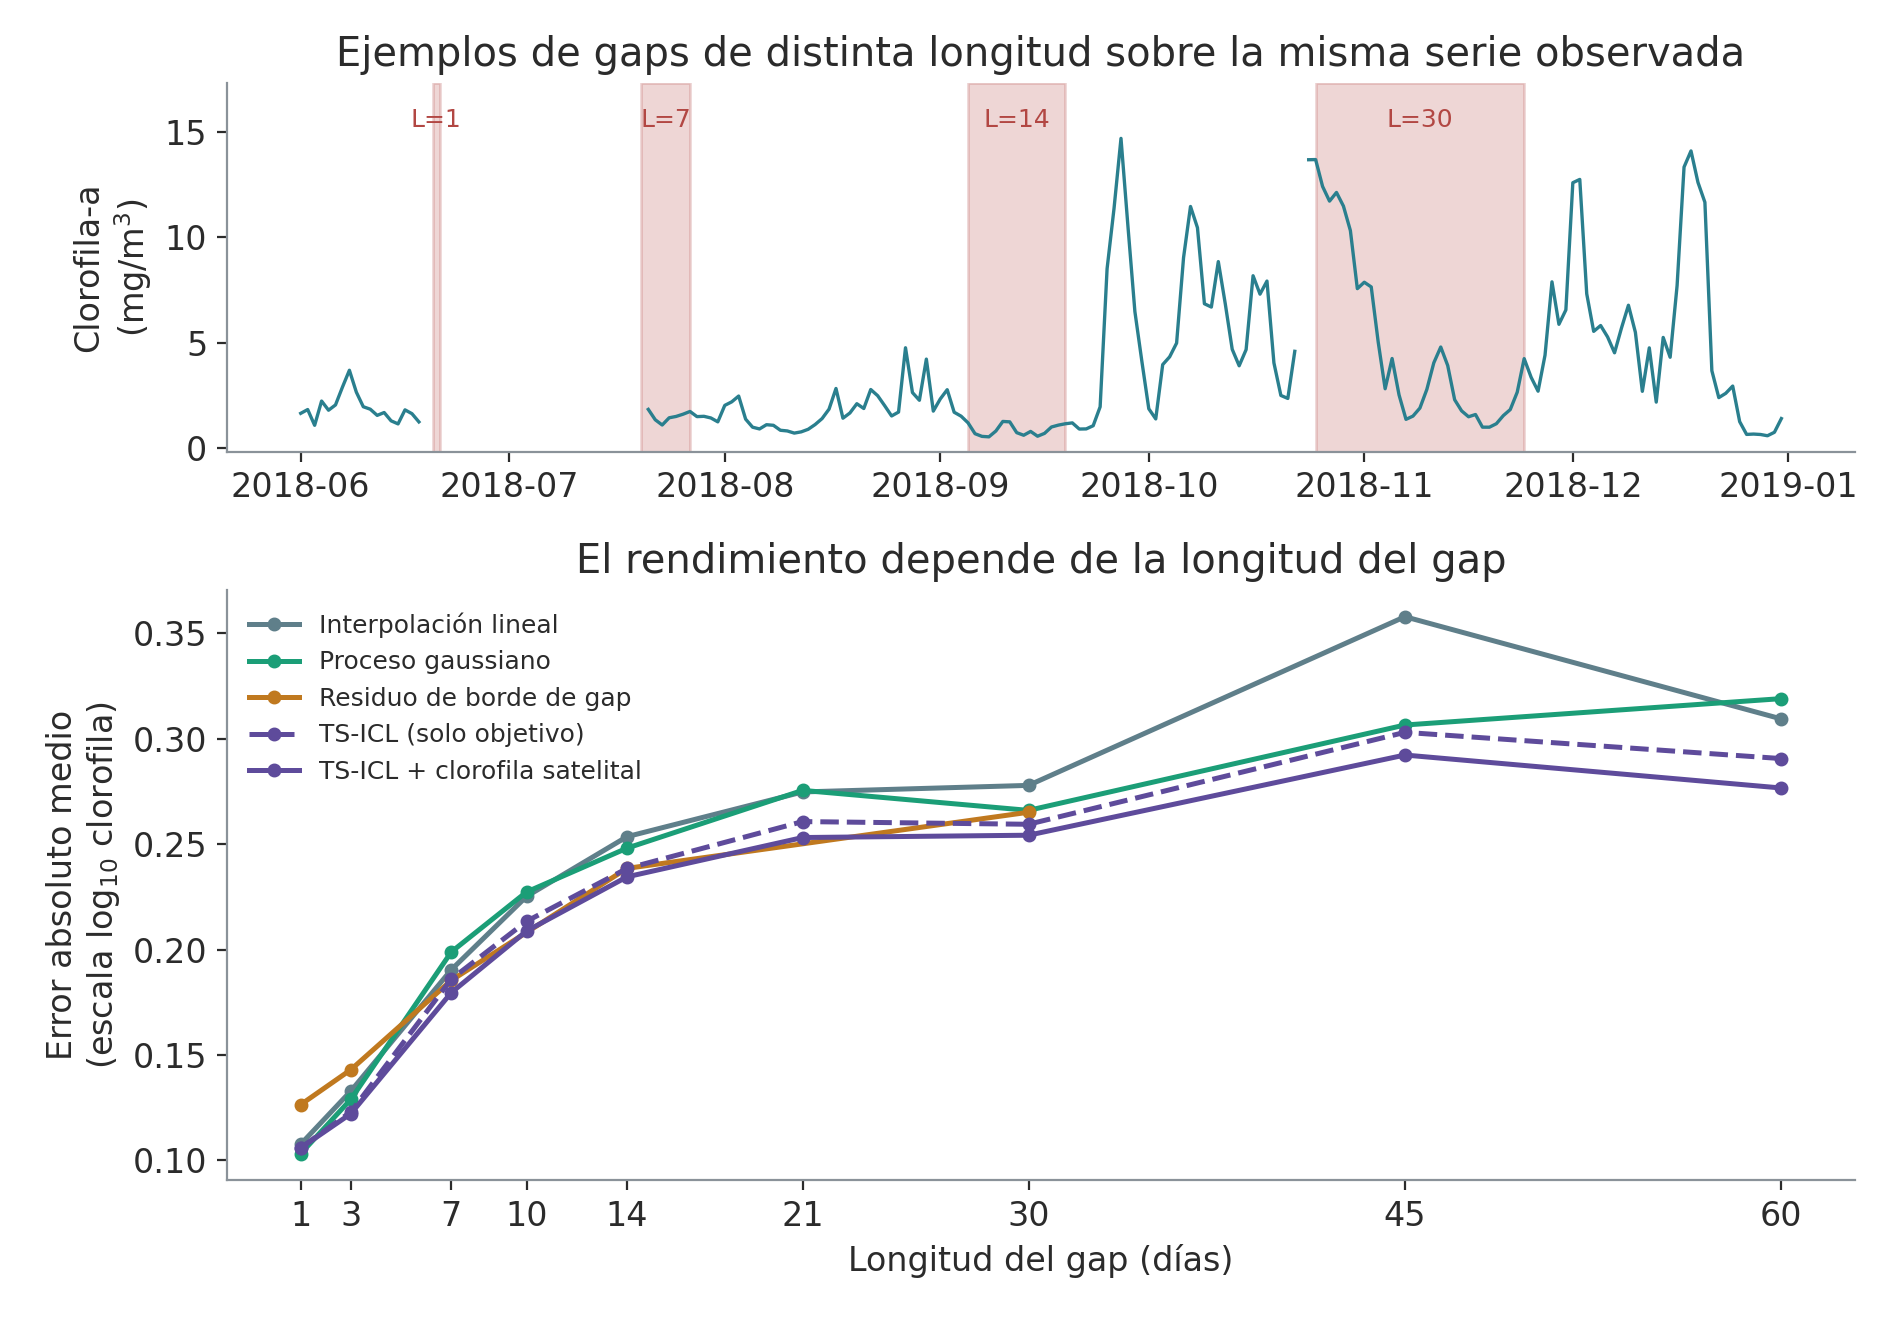
\includegraphics[width=0.50\textwidth]{figures/fig_f_gap_length_stratification.png}
  \end{center}
  \vskip1pt
  \takeaway{\footnotesize Un método puede ser competitivo en gaps cortos y perder esa
   ventaja a medida que el intervalo crece (y viceversa). Además del resumen agregado,
   el rendimiento debe examinarse \textbf{por longitud del gap}.}
\end{frame}

% ═══════════════ BLOQUE C --- QUÉ HACE CADA FAMILIA DE MÉTODOS ═══════════════

% ───────────────────────── DIAPOSITIVA 11 ─────────────────────────
\begin{frame}[t]{Familia 1: líneas de base simples}
  \vskip4pt
  \begin{columns}[T]
    \begin{column}{0.40\textwidth}
      \centering
      \adjustbox{max width=\linewidth,max height=6.4cm,center}{%% Recorte vectorial de una familia de metodos, generado a partir de
%% manuscript/presentation/figures/fig_model_ladder_tikz.tex (NO modificado).
%% Fuente compartida (colores, geometria, macros) copiada tal cual; solo se aisla
%% un panel y se traducen las tres etiquetas de fila.
\definecolor{vgTarget}{HTML}{2A7F8E}  % observed target (teal)
\definecolor{vgRecon}{HTML}{1B9E77}   % reconstruction / smoother output (green)
\definecolor{vgExt}{HTML}{3B6FA0}     % external predictors / features (blue)
\definecolor{vgEdge}{HTML}{D98A2B}    % gap-edge / residual correction (amber)
\definecolor{vgPrior}{HTML}{7E6CA8}   % TS-ICL / pretrained sequence model (violet)
\definecolor{vgHidden}{HTML}{C0504D}  % hidden gap (red)
\definecolor{vgInk}{HTML}{2B2B2B}     % text
\definecolor{vgFaint}{HTML}{9AA6B2}   % row tags / faint rules
\definecolor{vgGrid}{HTML}{D9DEE2}    % daily time grid
\definecolor{vgArrow}{HTML}{8A9299}   % flow arrows
\definecolor{vgPanel}{HTML}{F7F8F9}   % panel background
\definecolor{vgChip}{HTML}{ECEFF2}    % model chip fill

\definecolor{mBase}{HTML}{5F7F8A}     % simple baselines
\definecolor{mGP}{HTML}{1B9E77}       % Gaussian process
\definecolor{mExt}{HTML}{3B6FA0}      % external tabular
\definecolor{mGap}{HTML}{D98A2B}      % gap-edge residual
\definecolor{mTS}{HTML}{7E6CA8}       % TS-ICL
\definecolor{tsgreen}{HTML}{08A69B}
\definecolor{tsblue}{HTML}{004CF8}


\begin{tikzpicture}[x=0.38cm, y=0.38cm, font=\small,
    flow/.style={-{Latex[length=2mm]}, vgArrow, line width=0.9pt}]

  % ---------------------------------------------------------------------------
  % Global geometry
  % ---------------------------------------------------------------------------
  \def\PW{9.7}        % panel width
  \def\PH{24.9}       % panel height
  \def\DX{10.55}      % horizontal shift between panels

  \def\Ytitle{23.95}
  \def\YmodelA{20.60}
  \def\YmodelB{22.70}
  \def\YhowA{10.45}
  \def\YhowB{19.75}
  \def\YoutA{1.55}
  \def\YoutB{9.20}

  \def\Yeq{7.65}      % equation height inside output box
  \def\ob{2.95}       % baseline of output mini-plots

  % ---------------------------------------------------------------------------
  % Helpers
  % ---------------------------------------------------------------------------

  \newcommand{\panelbg}[2]{%
    \fill[vgPanel, rounded corners=3pt] (-0.25,0.75) rectangle (\PW,\PH);
    \draw[#2, opacity=0.45, line width=0.65pt, rounded corners=3pt]
      (-0.25,0.75) rectangle (\PW,\PH);
    \node[font=\small\bfseries, text=vgInk, align=center] at (4.72,\Ytitle) {#1};
  }

  \newcommand{\modelchip}[1]{%
    \fill[vgChip, rounded corners=3pt] (1.05,\YmodelA) rectangle (8.40,\YmodelB);
    \draw[#1, opacity=0.40, line width=0.55pt, rounded corners=3pt]
      (1.05,\YmodelA) rectangle (8.40,\YmodelB);
  }

  \newcommand{\howbox}[1]{%
    \fill[#1, opacity=0.040, rounded corners=3pt] (0.55,\YhowA) rectangle (8.95,\YhowB);
    \draw[#1, opacity=0.75, line width=0.7pt, rounded corners=3pt]
      (0.55,\YhowA) rectangle (8.95,\YhowB);
  }

  \newcommand{\outbox}[1]{%
    \fill[#1, opacity=0.040, rounded corners=3pt] (0.55,\YoutA) rectangle (8.95,\YoutB);
    \draw[#1, opacity=0.75, line width=0.7pt, rounded corners=3pt]
      (0.55,\YoutA) rectangle (8.95,\YoutB);
  }

  \newcommand{\imageorfallback}[3]{%
    \IfFileExists{#1}{%
      \includegraphics[width=#2]{#1}%
    }{%
      \fbox{\parbox[c][2.8cm][c]{#2}{\centering\scriptsize #3}}%
    }%
  }

  % output grid with observed context and hidden interval
  \newcommand{\miniout}[1]{%
    \foreach \s in {1,...,9}{
      \draw[vgGrid,line width=0.28pt](0.2+\s*0.9,#1)--(0.2+\s*0.9,#1+3.3);
    }
    \fill[vgHidden,opacity=0.12](0.2+3.5*0.9,#1)rectangle(0.2+6.5*0.9,#1+3.3);
    \draw[vgTarget,line width=1.0pt](1.1,#1+1.35)--(2.0,#1+1.00)--(2.9,#1+1.20);
    \draw[vgTarget,line width=1.0pt](6.5,#1+2.50)--(7.4,#1+2.85)--(8.3,#1+2.50);
    \foreach \s/\y in {1/1.35,2/1.00,3/1.20,7/2.50,8/2.85,9/2.50}{
      \fill[vgTarget](0.2+\s*0.9,#1+\y)circle(0.10);
    }
  }

  % compact target-gap sketch used in "how" boxes
  \newcommand{\howgap}[1]{%
    \foreach \s in {1,...,9}{
      \draw[vgGrid,line width=0.25pt](0.2+\s*0.9,#1)--(0.2+\s*0.9,#1+3.3);
    }
    \fill[vgHidden,opacity=0.12](0.2+3.5*0.9,#1)rectangle(0.2+6.5*0.9,#1+3.3);
    \draw[vgTarget,line width=0.95pt](1.1,#1+1.35)--(2.0,#1+1.00)--(2.9,#1+1.20);
    \draw[vgTarget,line width=0.95pt](6.5,#1+2.50)--(7.4,#1+2.85)--(8.3,#1+2.50);
    \foreach \s/\y in {1/1.35,2/1.00,3/1.20,7/2.50,8/2.85,9/2.50}{
      \fill[vgTarget](0.2+\s*0.9,#1+\y)circle(0.09);
    }
  }


  \node[rotate=90,font=\footnotesize\bfseries,text=vgFaint] at (-2.25,22.10) {MÉTODO};
  \node[rotate=90,font=\footnotesize\bfseries,text=vgFaint] at (-2.25,15.10) {MECANISMO};
  \node[rotate=90,font=\footnotesize\bfseries,text=vgFaint] at (-2.25,5.35) {SALIDA};

  % ---------------------------------------------------------------------------
  \begin{scope}[shift={(0,0)}]
    \panelbg{Líneas de base simples}{mBase}
    \modelchip{mBase}
    \node[font=\tiny, text=vgInk, align=center, text width=3.2cm] at (4.72,21.65)
      {climatología\\persistencia\\interpolación lineal};

    \howbox{mBase}
    % three rule sketches with equations, not names
    \def\yshift{-0.9}
\foreach \yy/\eqn in {
  17.90/{{$\hat y_t = y_{t^-}$}},
  15.90/{{$\hat y_t=\tilde y_t^{\mathrm{lin}}$}},
  13.90/{{$\hat y_t = \mu_{\mathrm{season}}$}}
}{
  \fill[vgHidden,opacity=0.12](1.35,\yy-0.55+\yshift) rectangle (2.30,\yy+0.55+\yshift);
  \fill[vgTarget](0.95,\yy-0.25+\yshift) circle(0.09);
  \fill[vgTarget](2.80,\yy+0.30+\yshift) circle(0.09);
  \node[font=\scriptsize,text=vgInk,anchor=west] at (3.60,\yy+\yshift) {\eqn};
}
    % persistence
    \draw[mBase,line width=1.35pt] (0.95,16.75)--(2.80,16.75);
    % interpolation
    \draw[mBase,line width=1.35pt] (0.95,14.75)--(2.80,15.30);
    % climatology
    \draw[mBase,line width=1.35pt] (0.95,13)--(2.80,13);

    \draw[flow] (4.75,20.35)--(4.75,19.95);
    \draw[flow] (4.75,10.25)--(4.75,9.55);

    \outbox{mBase}
    \node[font=\scriptsize,text=vgInk,align=center] at (4.75,\Yeq)
      {$\hat y_t=\tilde y_t^{\mathrm{lin}}$};
    \miniout{\ob}
    % only interpolation shown in output
    \draw[mBase,line width=1.6pt](2.9,\ob+1.2)--(6.5,\ob+2.5);
    \foreach \s in {4,5,6}{
      \fill[mBase](0.2+\s*0.9,{\ob+1.2+(\s-3)*0.325})circle(0.10);
    }
  \end{scope}
\end{tikzpicture}
}
    \end{column}
    \begin{column}{0.56\textwidth}
      \vskip0.3cm
      {\footnotesize
      \begin{itemize}\setlength\itemsep{0.20cm}
        \item Sin ajuste local: se calculan en el momento, sin entrenar nada.
        \item Sorprendentemente difíciles de superar en gaps cortos y medianos.
        \item La implementación usada en el reporte entrega un valor puntual, sin banda
          de incertidumbre.
        \item Referencia obligatoria: cualquier método más complejo debe justificar por
          qué vale la pena frente a esto.
      \end{itemize}}
    \end{column}
  \end{columns}
\end{frame}

% ───────────────────────── DIAPOSITIVA 12 ─────────────────────────
\begin{frame}[t]{Familia 2: suavizado solo-objetivo}
  \vskip4pt
  \begin{columns}[T]
    \begin{column}{0.40\textwidth}
      \centering
      \adjustbox{max width=\linewidth,max height=6.4cm,center}{%% Recorte vectorial de una familia de metodos, generado a partir de
%% manuscript/presentation/figures/fig_model_ladder_tikz.tex (NO modificado).
%% Fuente compartida (colores, geometria, macros) copiada tal cual; solo se aisla
%% un panel y se traducen las tres etiquetas de fila.
\definecolor{vgTarget}{HTML}{2A7F8E}  % observed target (teal)
\definecolor{vgRecon}{HTML}{1B9E77}   % reconstruction / smoother output (green)
\definecolor{vgExt}{HTML}{3B6FA0}     % external predictors / features (blue)
\definecolor{vgEdge}{HTML}{D98A2B}    % gap-edge / residual correction (amber)
\definecolor{vgPrior}{HTML}{7E6CA8}   % TS-ICL / pretrained sequence model (violet)
\definecolor{vgHidden}{HTML}{C0504D}  % hidden gap (red)
\definecolor{vgInk}{HTML}{2B2B2B}     % text
\definecolor{vgFaint}{HTML}{9AA6B2}   % row tags / faint rules
\definecolor{vgGrid}{HTML}{D9DEE2}    % daily time grid
\definecolor{vgArrow}{HTML}{8A9299}   % flow arrows
\definecolor{vgPanel}{HTML}{F7F8F9}   % panel background
\definecolor{vgChip}{HTML}{ECEFF2}    % model chip fill

\definecolor{mBase}{HTML}{5F7F8A}     % simple baselines
\definecolor{mGP}{HTML}{1B9E77}       % Gaussian process
\definecolor{mExt}{HTML}{3B6FA0}      % external tabular
\definecolor{mGap}{HTML}{D98A2B}      % gap-edge residual
\definecolor{mTS}{HTML}{7E6CA8}       % TS-ICL
\definecolor{tsgreen}{HTML}{08A69B}
\definecolor{tsblue}{HTML}{004CF8}


\begin{tikzpicture}[x=0.38cm, y=0.38cm, font=\small,
    flow/.style={-{Latex[length=2mm]}, vgArrow, line width=0.9pt}]

  % ---------------------------------------------------------------------------
  % Global geometry
  % ---------------------------------------------------------------------------
  \def\PW{9.7}        % panel width
  \def\PH{24.9}       % panel height
  \def\DX{10.55}      % horizontal shift between panels

  \def\Ytitle{23.95}
  \def\YmodelA{20.60}
  \def\YmodelB{22.70}
  \def\YhowA{10.45}
  \def\YhowB{19.75}
  \def\YoutA{1.55}
  \def\YoutB{9.20}

  \def\Yeq{7.65}      % equation height inside output box
  \def\ob{2.95}       % baseline of output mini-plots

  % ---------------------------------------------------------------------------
  % Helpers
  % ---------------------------------------------------------------------------

  \newcommand{\panelbg}[2]{%
    \fill[vgPanel, rounded corners=3pt] (-0.25,0.75) rectangle (\PW,\PH);
    \draw[#2, opacity=0.45, line width=0.65pt, rounded corners=3pt]
      (-0.25,0.75) rectangle (\PW,\PH);
    \node[font=\small\bfseries, text=vgInk, align=center] at (4.72,\Ytitle) {#1};
  }

  \newcommand{\modelchip}[1]{%
    \fill[vgChip, rounded corners=3pt] (1.05,\YmodelA) rectangle (8.40,\YmodelB);
    \draw[#1, opacity=0.40, line width=0.55pt, rounded corners=3pt]
      (1.05,\YmodelA) rectangle (8.40,\YmodelB);
  }

  \newcommand{\howbox}[1]{%
    \fill[#1, opacity=0.040, rounded corners=3pt] (0.55,\YhowA) rectangle (8.95,\YhowB);
    \draw[#1, opacity=0.75, line width=0.7pt, rounded corners=3pt]
      (0.55,\YhowA) rectangle (8.95,\YhowB);
  }

  \newcommand{\outbox}[1]{%
    \fill[#1, opacity=0.040, rounded corners=3pt] (0.55,\YoutA) rectangle (8.95,\YoutB);
    \draw[#1, opacity=0.75, line width=0.7pt, rounded corners=3pt]
      (0.55,\YoutA) rectangle (8.95,\YoutB);
  }

  \newcommand{\imageorfallback}[3]{%
    \IfFileExists{#1}{%
      \includegraphics[width=#2]{#1}%
    }{%
      \fbox{\parbox[c][2.8cm][c]{#2}{\centering\scriptsize #3}}%
    }%
  }

  % output grid with observed context and hidden interval
  \newcommand{\miniout}[1]{%
    \foreach \s in {1,...,9}{
      \draw[vgGrid,line width=0.28pt](0.2+\s*0.9,#1)--(0.2+\s*0.9,#1+3.3);
    }
    \fill[vgHidden,opacity=0.12](0.2+3.5*0.9,#1)rectangle(0.2+6.5*0.9,#1+3.3);
    \draw[vgTarget,line width=1.0pt](1.1,#1+1.35)--(2.0,#1+1.00)--(2.9,#1+1.20);
    \draw[vgTarget,line width=1.0pt](6.5,#1+2.50)--(7.4,#1+2.85)--(8.3,#1+2.50);
    \foreach \s/\y in {1/1.35,2/1.00,3/1.20,7/2.50,8/2.85,9/2.50}{
      \fill[vgTarget](0.2+\s*0.9,#1+\y)circle(0.10);
    }
  }

  % compact target-gap sketch used in "how" boxes
  \newcommand{\howgap}[1]{%
    \foreach \s in {1,...,9}{
      \draw[vgGrid,line width=0.25pt](0.2+\s*0.9,#1)--(0.2+\s*0.9,#1+3.3);
    }
    \fill[vgHidden,opacity=0.12](0.2+3.5*0.9,#1)rectangle(0.2+6.5*0.9,#1+3.3);
    \draw[vgTarget,line width=0.95pt](1.1,#1+1.35)--(2.0,#1+1.00)--(2.9,#1+1.20);
    \draw[vgTarget,line width=0.95pt](6.5,#1+2.50)--(7.4,#1+2.85)--(8.3,#1+2.50);
    \foreach \s/\y in {1/1.35,2/1.00,3/1.20,7/2.50,8/2.85,9/2.50}{
      \fill[vgTarget](0.2+\s*0.9,#1+\y)circle(0.09);
    }
  }


  \node[rotate=90,font=\footnotesize\bfseries,text=vgFaint] at (-2.25,22.10) {MÉTODO};
  \node[rotate=90,font=\footnotesize\bfseries,text=vgFaint] at (-2.25,15.10) {MECANISMO};
  \node[rotate=90,font=\footnotesize\bfseries,text=vgFaint] at (-2.25,5.35) {SALIDA};

  % ---------------------------------------------------------------------------
  \begin{scope}[shift={(\DX,0)}]
    \panelbg{\scalebox{0.85}{Suavizado solo-objetivo}}{mGP}
    \modelchip{mGP}
    \node[font=\scriptsize, text=vgInk, align=center, text width=3.0cm] at (4.72,21.65)
      {Proceso gaussiano};

    \howbox{mGP}

\begin{scope}[yshift=-0.35cm]
\howgap{13.85}

% Prior mean m(t): faint dashed reference trend
\draw[vgFaint,line width=0.75pt,dash pattern=on 2pt off 1.5pt]
  plot[smooth] coordinates{
    (1.1,15.20)
    (2.9,15.10)
    (4.7,15.70)
    (6.5,16.35)
    (8.3,16.25)
  };
\node[font=\scriptsize,text=vgFaint,anchor=west] at (6.75,14.75) {$m(t)$};

% Posterior uncertainty induced by the covariance kernel inside/near the gap
\fill[mGP,opacity=0.13]
  plot[smooth] coordinates{
    (2.9,15.32)
    (3.6,15.55)
    (4.7,16.25)
    (5.8,16.55)
    (6.5,16.58)
  }
  -- plot[smooth] coordinates{
    (6.5,16.12)
    (5.8,15.55)
    (4.7,15.05)
    (3.6,14.92)
    (2.9,14.92)
  }
  -- cycle;

% Posterior mean reconstruction
\draw[mGP,line width=1.65pt]
  plot[smooth] coordinates{
    (2.9,15.05)
    (3.6,15.18)
    (4.7,15.75)
    (5.8,16.12)
    (6.5,16.35)
  };

% Small covariance cue
\draw[mGP,line width=0.55pt,opacity=0.85]
  (4.15,16.15) to[bend left=30] (5.25,16.15);
\draw[mGP,line width=0.55pt,opacity=0.65]
  (3.80,16.42) to[bend left=35] (5.60,16.42);
\node[font=\scriptsize,text=mGP] at (4.70,17.80) {$k(t,t')$};
\end{scope}

\draw[flow] (4.75,20.35)--(4.75,19.95);
\draw[flow] (4.75,10.25)--(4.75,9.55);

    \outbox{mGP}
    \node[font=\scriptsize,text=vgInk,align=center] at (4.75,\Yeq)
      {$\hat y(t)\sim\mathcal{GP}(m,k)$};
    \miniout{\ob}
    \fill[mGP,opacity=0.14]
      plot[smooth]coordinates{(2.9,\ob+1.25)(3.8,\ob+1.20)(4.7,\ob+2.75)(5.6,\ob+2.25)(6.5,\ob+2.55)}
      --plot[smooth]coordinates{(6.5,\ob+2.45)(5.6,\ob+1.55)(4.7,\ob+2.00)(3.8,\ob+0.60)(2.9,\ob+1.15)}
      --cycle;
    \draw[mGP,line width=1.6pt]
      plot[smooth]coordinates{(2.9,\ob+1.20)(3.8,\ob+0.90)(4.7,\ob+2.40)(5.6,\ob+1.90)(6.5,\ob+2.50)};
  \end{scope}
\end{tikzpicture}
}
    \end{column}
    \begin{column}{0.56\textwidth}
      \vskip0.3cm
      {\footnotesize
      \begin{itemize}\setlength\itemsep{0.20cm}
        \item Usa solo la estructura temporal de la propia variable, sin covariables.
        \item Se ajusta a la serie local; asume que valores cercanos en el tiempo se
          parecen, con una escala de correlación aprendida de los datos.
        \item Entrega una banda \textbf{predictiva/posterior} alrededor de la
          reconstrucción --- no es una ``banda de confianza'' genérica, es la
          incertidumbre del propio modelo probabilístico.
        \item Puede perder el evento si la variable cambia de régimen dentro del gap: la
          suavidad es una suposición, no una garantía.
      \end{itemize}}
    \end{column}
  \end{columns}
\end{frame}

% ───────────────────────── DIAPOSITIVA 13 ─────────────────────────
\begin{frame}[t]{Familia 3: tabular con variables externas}
  \vskip4pt
  \begin{columns}[T]
    \begin{column}{0.40\textwidth}
      \centering
      \adjustbox{max width=\linewidth,max height=6.4cm,center}{%% Recorte vectorial de una familia de metodos, generado a partir de
%% manuscript/presentation/figures/fig_model_ladder_tikz.tex (NO modificado).
%% Fuente compartida (colores, geometria, macros) copiada tal cual; solo se aisla
%% un panel y se traducen las tres etiquetas de fila.
\definecolor{vgTarget}{HTML}{2A7F8E}  % observed target (teal)
\definecolor{vgRecon}{HTML}{1B9E77}   % reconstruction / smoother output (green)
\definecolor{vgExt}{HTML}{3B6FA0}     % external predictors / features (blue)
\definecolor{vgEdge}{HTML}{D98A2B}    % gap-edge / residual correction (amber)
\definecolor{vgPrior}{HTML}{7E6CA8}   % TS-ICL / pretrained sequence model (violet)
\definecolor{vgHidden}{HTML}{C0504D}  % hidden gap (red)
\definecolor{vgInk}{HTML}{2B2B2B}     % text
\definecolor{vgFaint}{HTML}{9AA6B2}   % row tags / faint rules
\definecolor{vgGrid}{HTML}{D9DEE2}    % daily time grid
\definecolor{vgArrow}{HTML}{8A9299}   % flow arrows
\definecolor{vgPanel}{HTML}{F7F8F9}   % panel background
\definecolor{vgChip}{HTML}{ECEFF2}    % model chip fill

\definecolor{mBase}{HTML}{5F7F8A}     % simple baselines
\definecolor{mGP}{HTML}{1B9E77}       % Gaussian process
\definecolor{mExt}{HTML}{3B6FA0}      % external tabular
\definecolor{mGap}{HTML}{D98A2B}      % gap-edge residual
\definecolor{mTS}{HTML}{7E6CA8}       % TS-ICL
\definecolor{tsgreen}{HTML}{08A69B}
\definecolor{tsblue}{HTML}{004CF8}


\begin{tikzpicture}[x=0.38cm, y=0.38cm, font=\small,
    flow/.style={-{Latex[length=2mm]}, vgArrow, line width=0.9pt}]

  % ---------------------------------------------------------------------------
  % Global geometry
  % ---------------------------------------------------------------------------
  \def\PW{9.7}        % panel width
  \def\PH{24.9}       % panel height
  \def\DX{10.55}      % horizontal shift between panels

  \def\Ytitle{23.95}
  \def\YmodelA{20.60}
  \def\YmodelB{22.70}
  \def\YhowA{10.45}
  \def\YhowB{19.75}
  \def\YoutA{1.55}
  \def\YoutB{9.20}

  \def\Yeq{7.65}      % equation height inside output box
  \def\ob{2.95}       % baseline of output mini-plots

  % ---------------------------------------------------------------------------
  % Helpers
  % ---------------------------------------------------------------------------

  \newcommand{\panelbg}[2]{%
    \fill[vgPanel, rounded corners=3pt] (-0.25,0.75) rectangle (\PW,\PH);
    \draw[#2, opacity=0.45, line width=0.65pt, rounded corners=3pt]
      (-0.25,0.75) rectangle (\PW,\PH);
    \node[font=\small\bfseries, text=vgInk, align=center] at (4.72,\Ytitle) {#1};
  }

  \newcommand{\modelchip}[1]{%
    \fill[vgChip, rounded corners=3pt] (1.05,\YmodelA) rectangle (8.40,\YmodelB);
    \draw[#1, opacity=0.40, line width=0.55pt, rounded corners=3pt]
      (1.05,\YmodelA) rectangle (8.40,\YmodelB);
  }

  \newcommand{\howbox}[1]{%
    \fill[#1, opacity=0.040, rounded corners=3pt] (0.55,\YhowA) rectangle (8.95,\YhowB);
    \draw[#1, opacity=0.75, line width=0.7pt, rounded corners=3pt]
      (0.55,\YhowA) rectangle (8.95,\YhowB);
  }

  \newcommand{\outbox}[1]{%
    \fill[#1, opacity=0.040, rounded corners=3pt] (0.55,\YoutA) rectangle (8.95,\YoutB);
    \draw[#1, opacity=0.75, line width=0.7pt, rounded corners=3pt]
      (0.55,\YoutA) rectangle (8.95,\YoutB);
  }

  \newcommand{\imageorfallback}[3]{%
    \IfFileExists{#1}{%
      \includegraphics[width=#2]{#1}%
    }{%
      \fbox{\parbox[c][2.8cm][c]{#2}{\centering\scriptsize #3}}%
    }%
  }

  % output grid with observed context and hidden interval
  \newcommand{\miniout}[1]{%
    \foreach \s in {1,...,9}{
      \draw[vgGrid,line width=0.28pt](0.2+\s*0.9,#1)--(0.2+\s*0.9,#1+3.3);
    }
    \fill[vgHidden,opacity=0.12](0.2+3.5*0.9,#1)rectangle(0.2+6.5*0.9,#1+3.3);
    \draw[vgTarget,line width=1.0pt](1.1,#1+1.35)--(2.0,#1+1.00)--(2.9,#1+1.20);
    \draw[vgTarget,line width=1.0pt](6.5,#1+2.50)--(7.4,#1+2.85)--(8.3,#1+2.50);
    \foreach \s/\y in {1/1.35,2/1.00,3/1.20,7/2.50,8/2.85,9/2.50}{
      \fill[vgTarget](0.2+\s*0.9,#1+\y)circle(0.10);
    }
  }

  % compact target-gap sketch used in "how" boxes
  \newcommand{\howgap}[1]{%
    \foreach \s in {1,...,9}{
      \draw[vgGrid,line width=0.25pt](0.2+\s*0.9,#1)--(0.2+\s*0.9,#1+3.3);
    }
    \fill[vgHidden,opacity=0.12](0.2+3.5*0.9,#1)rectangle(0.2+6.5*0.9,#1+3.3);
    \draw[vgTarget,line width=0.95pt](1.1,#1+1.35)--(2.0,#1+1.00)--(2.9,#1+1.20);
    \draw[vgTarget,line width=0.95pt](6.5,#1+2.50)--(7.4,#1+2.85)--(8.3,#1+2.50);
    \foreach \s/\y in {1/1.35,2/1.00,3/1.20,7/2.50,8/2.85,9/2.50}{
      \fill[vgTarget](0.2+\s*0.9,#1+\y)circle(0.09);
    }
  }


  \node[rotate=90,font=\footnotesize\bfseries,text=vgFaint] at (-2.25,22.10) {MÉTODO};
  \node[rotate=90,font=\footnotesize\bfseries,text=vgFaint] at (-2.25,15.10) {MECANISMO};
  \node[rotate=90,font=\footnotesize\bfseries,text=vgFaint] at (-2.25,5.35) {SALIDA};

  % ---------------------------------------------------------------------------
  \begin{scope}[shift={(0,0)}]
    \panelbg{Tabular externo}{mExt}
    \modelchip{mExt}
    \node[font=\scriptsize, text=vgInk, align=center, text width=3.0cm] at (4.72,21.65)
      {HGB, ExtraTrees};

    \howbox{mExt}
    % mecanismo: construccion explicita de variables, un vector por dia
    \node[font=\tiny,text=vgInk,align=center,text width=3.0cm] at (4.75,18.55)
      {objetivo + covariables diarias};
    \draw[flow,line width=0.7pt] (4.75,17.55)--(4.75,16.95);
    \node[font=\tiny,text=vgInk,align=center,text width=3.15cm] at (4.75,15.55)
      {calendario, rezagos, promedios móviles, índices acumulados};
    \draw[flow,line width=0.7pt] (4.75,13.95)--(4.75,13.35);
    \node[font=\scriptsize,text=mExt,align=center,text width=3.0cm] at (4.75,12.35)
      {vector de variables $\phi_t$\\(uno por dia)};

    \draw[flow] (4.75,20.35)--(4.75,19.95);
    \draw[flow] (4.75,10.25)--(4.75,9.55);

    \outbox{mExt}
    \node[font=\scriptsize,text=vgInk,align=center] at (4.75,\Yeq)
      {$\hat y_t = f(\phi_t)$};
    \miniout{\ob}
    \foreach \s/\y in {4/1.35,5/1.90,6/1.55}{
      \fill[mExt](0.2+\s*0.9,\ob+\y)circle(0.15);
    }
  \end{scope}
\end{tikzpicture}
}
    \end{column}
    \begin{column}{0.56\textwidth}
      \vskip0.3cm
      {\footnotesize
      \begin{itemize}\setlength\itemsep{0.18cm}
        \item Usa solo covariables (calendario, viento, temperatura superficial,
          clorofila satelital, etc.) --- \textbf{no} usa la trayectoria reciente del
          propio objetivo.
        \item Requiere construir variables explícitamente: rezagos, promedios móviles,
          índices acumulados.
        \item Requiere ajuste local con datos de esta estación.
        \item Hallazgo del proyecto: usado solo, quedó \textbf{por debajo de la
          interpolación} como reconstructor directo, tanto para clorofila como para
          oxígeno (ver casos más adelante).
      \end{itemize}}
    \end{column}
  \end{columns}
\end{frame}

% ───────────────────────── DIAPOSITIVA 14 ─────────────────────────
\begin{frame}[t]{Familia 4: residuo en el borde del gap}
  \vskip4pt
  \begin{columns}[T]
    \begin{column}{0.40\textwidth}
      \centering
      \adjustbox{max width=\linewidth,max height=6.4cm,center}{\input{figures/gap_edge_crop.tex}}
    \end{column}
    \begin{column}{0.56\textwidth}
      \vskip0.3cm
      {\footnotesize
      \begin{itemize}\setlength\itemsep{0.18cm}
        \item Parte de la interpolación lineal y aprende una corrección usando el
          contexto y \textbf{ambos bordes} del gap (antes y después) como insumos de
          reconstrucción.
        \item No usa el borde posterior solo ``para entrenar'' un modelo global: lo usa
          como \textbf{contexto de reconstrucción de ese gap específico}.
        \item Ayuda sobre todo en gaps \textbf{largos}, donde la interpolación simple
          pierde más precisión.
        \item Consecuencia directa: es retrospectivo, no aplicable en la misma forma a un
          gap abierto sin observaciones posteriores.
      \end{itemize}}
    \end{column}
  \end{columns}
\end{frame}

% ───────────────────────── DIAPOSITIVA 15 ─────────────────────────
\begin{frame}[t]{Familia 5: TS-ICL, un modelo preentrenado}
  \vskip4pt
  \begin{columns}[T]
    \begin{column}{0.34\textwidth}
      \vskip0.1cm
      \centering
      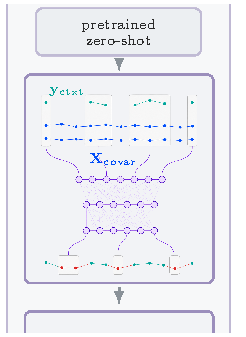
\includegraphics[width=0.92\linewidth]{figures/tsicl_architecture_crop.pdf}
    \end{column}
    \begin{column}{0.62\textwidth}
      \vskip0.05cm
      {\footnotesize
      \begin{itemize}\setlength\itemsep{0.16cm}
        \item Modelo de series temporales entrenado \textbf{una sola vez}, en muchas
          series distintas, en otro lugar.
        \item Se usa \textbf{zero-shot}: sin volver a entrenar ni ajustar con datos de
          Tongoy.
        \item Corre \textbf{solo-objetivo} (sin covariables) o \textbf{con covariables}
          como canales alineados en el tiempo --- las covariables son opcionales, no un
          requisito.
        \item Salida: reconstrucción puntual \textbf{y} cuantiles (banda q05--q95).
      \end{itemize}}
    \end{column}
  \end{columns}
  \vskip0.15cm
  {\scriptsize\color{faint}TS-ICL: Le Naour, Nabil \& Petralia (2026); paquete público
   \texttt{tsicl} (PyPI), EDF Lab.}
\end{frame}

% ───────────────────────── DIAPOSITIVA 16 ─────────────────────────
\begin{frame}[t]{Ventajas prácticas de TS-ICL, medidas en esta laptop}
  \vskip3pt
  {\small
  \begin{itemize}\setlength\itemsep{0.11cm}
    \item \textbf{Sin entrenamiento ni ajuste fino local}: el mismo modelo preentrenado
      puede aplicarse a una nueva serie sin ajuste fino local, pero debe volver a
      validarse en esa serie.
    \item \textbf{Inferencia rápida tras cargar el modelo}: en esta laptop (CPU, sin GPU),
      cargar el modelo toma bajo 1 segundo (checkpoint ya en caché) y cada reconstrucción
      sobre una ventana de \textasciitilde 5 meses toma \textasciitilde 0.05--0.1 s;
      sobre la serie completa (\textasciitilde 11 años) toma \textasciitilde 3 s.
    \item \textbf{Entrada solo-objetivo o con covariables}, sin cambiar de modelo.
    \item \textbf{Menos ingeniería manual de contexto temporal} que el enfoque tabular.
    \item \textbf{Salida probabilística} (cuantiles), no solo un número.
  \end{itemize}}
  \vskip0.12cm
  \caution{\footnotesize Esto no reemplaza la validación: el rendimiento de TS-ICL se
   sigue evaluando por longitud de gap y por régimen. Tampoco elimina el trabajo de
   elegir, alinear y controlar la calidad de las covariables que se le pasan.}
\end{frame}

% ───────────────────────── DIAPOSITIVA 17 ─────────────────────────
\begin{frame}[t]{Las cinco familias, una sola escalera}
  \vskip2pt
  \begin{center}
    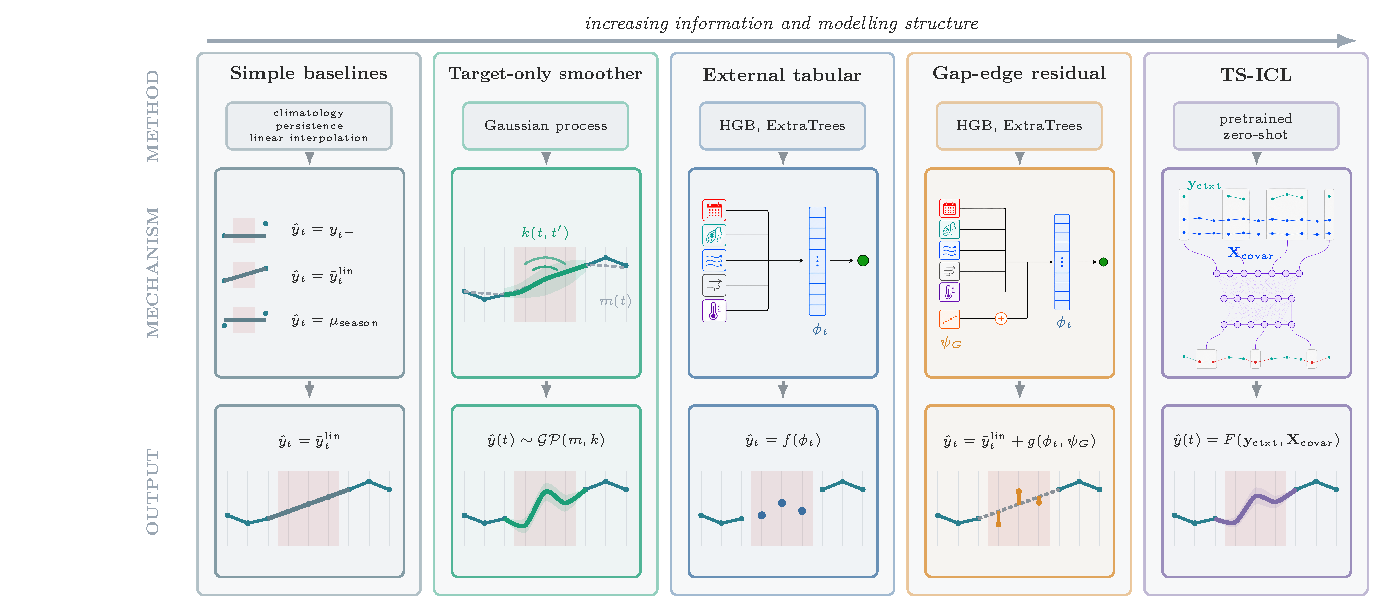
\includegraphics[width=0.90\textwidth]{figures/model_ladder_report.pdf}
  \end{center}
  \vskip2pt
  {\footnotesize\color{ink}Recapitulación: cada familia representa el contexto temporal de
   forma distinta; todas se evalúan con el mismo protocolo de gaps artificiales.}
\end{frame}

% ═══════════════ BLOQUE D --- QUÉ OCURRIÓ EN TONGOY ═══════════════

% ───────────────────────── DIAPOSITIVA 18 ─────────────────────────
\begin{frame}[t]{Caso clorofila: qué aprendimos}
  \vskip2pt
  \begin{center}
    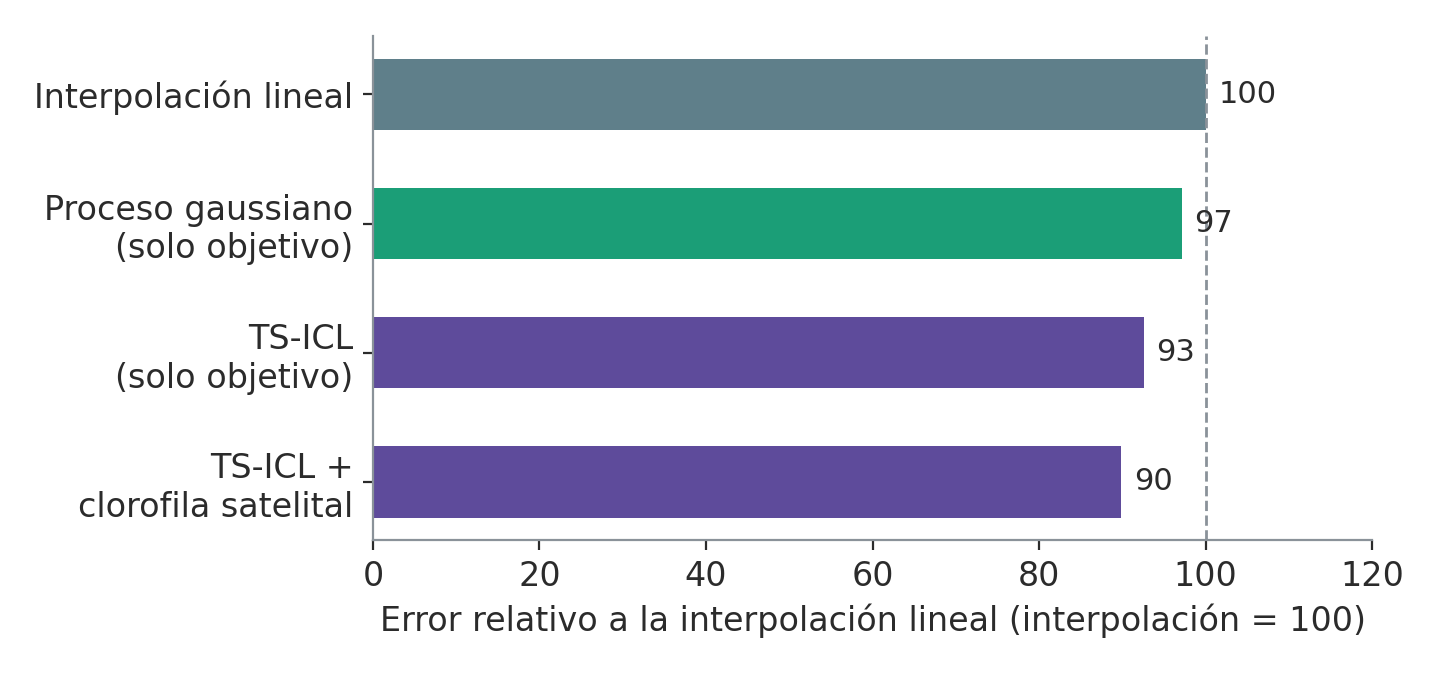
\includegraphics[width=0.56\textwidth]{figures/fig_b_chl_pooled_comparison.png}
  \end{center}
  \vskip2pt
  {\footnotesize\color{ink}
  \begin{itemize}\setlength\itemsep{0.05cm}
    \item La interpolación es una referencia difícil de superar.
    \item El tabular externo (solo covariables) queda por debajo de la interpolación.
    \item TS-ICL con clorofila satelital como covariable es, en promedio, el mejor
      candidato sobre el conjunto evaluado.
    \item Mejora moderada frente a comparadores que sí usan el objetivo (GP, TS-ICL
      solo-objetivo) --- no un cambio de orden de magnitud.
  \end{itemize}}
\end{frame}

% ───────────────────────── DIAPOSITIVA 19 ─────────────────────────
\begin{frame}[t]{Caso clorofila: la limitación de los eventos}
  \vskip1pt
  \begin{center}
    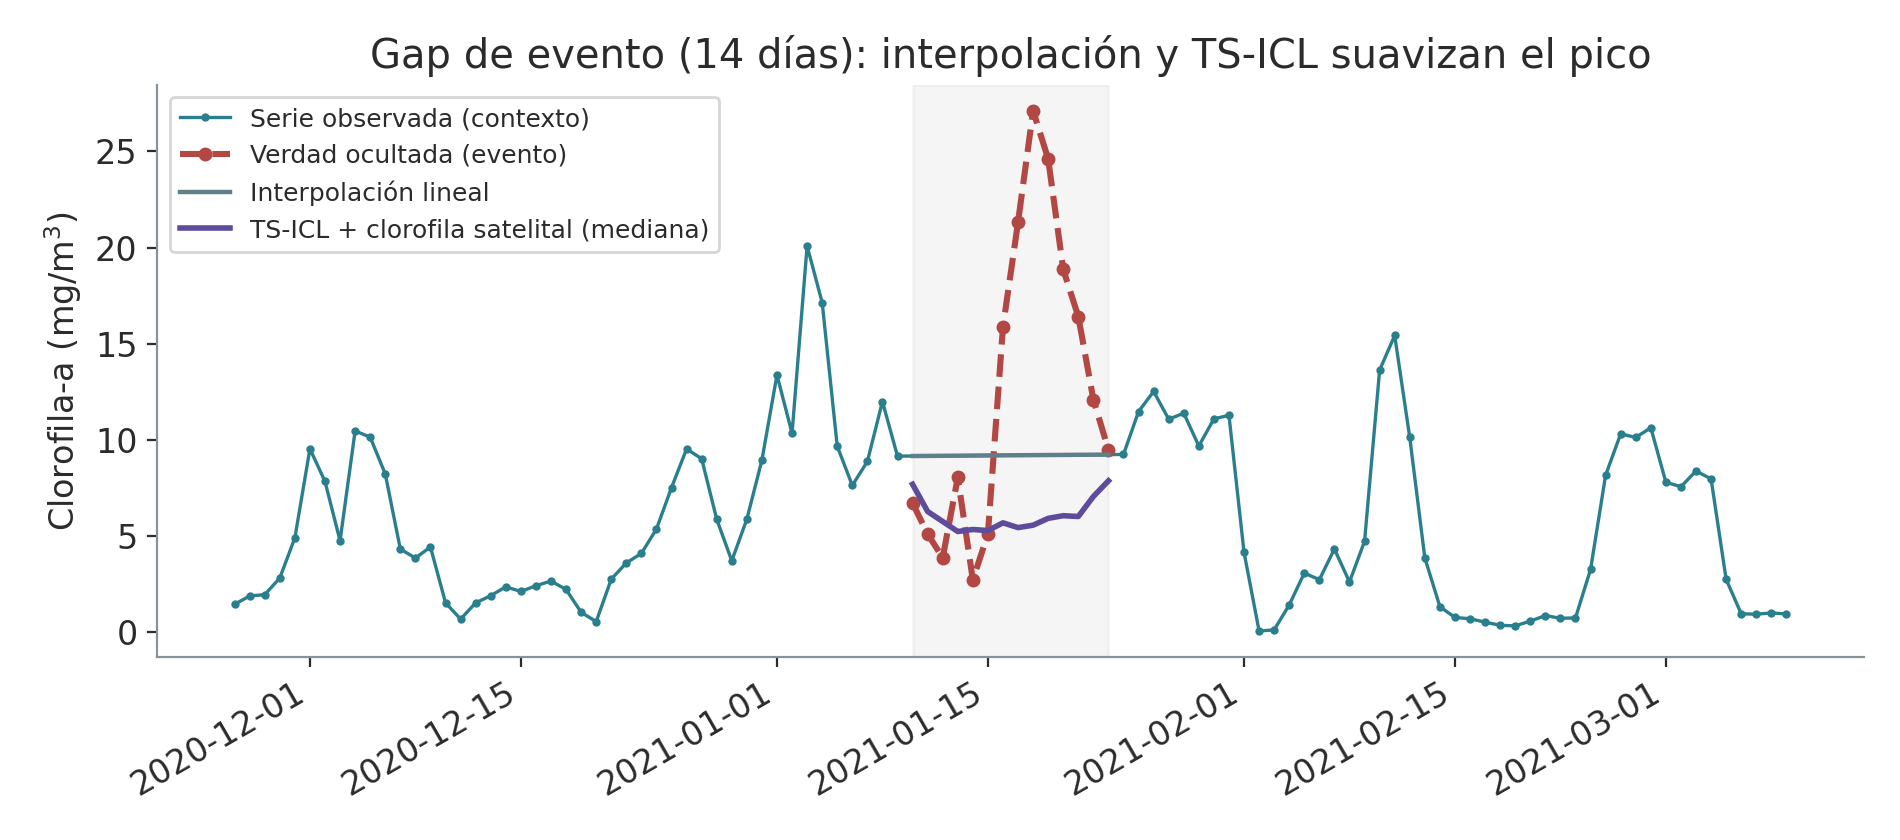
\includegraphics[width=0.50\textwidth]{figures/fig_g_chl_event_illustration.png}
  \end{center}
  \vskip1pt
  {\footnotesize\color{ink}\textbf{Gap de evento} = contiene al menos un día oculto por
   encima del percentil 90 empírico de clorofila. Interpolación y TS-ICL aplanan el pico
   real: ninguno anticipa la floración.}
  \vskip0.1cm
  \caution{\footnotesize\centering Patrón repetido en el conjunto evaluado: todos los
   métodos tienen más error en días de evento que en días normales.}
\end{frame}

% ───────────────────────── DIAPOSITIVA 20 ─────────────────────────
\begin{frame}[t]{Caso oxígeno: el mismo flujo transfiere}
  \vskip2pt
  \begin{center}
    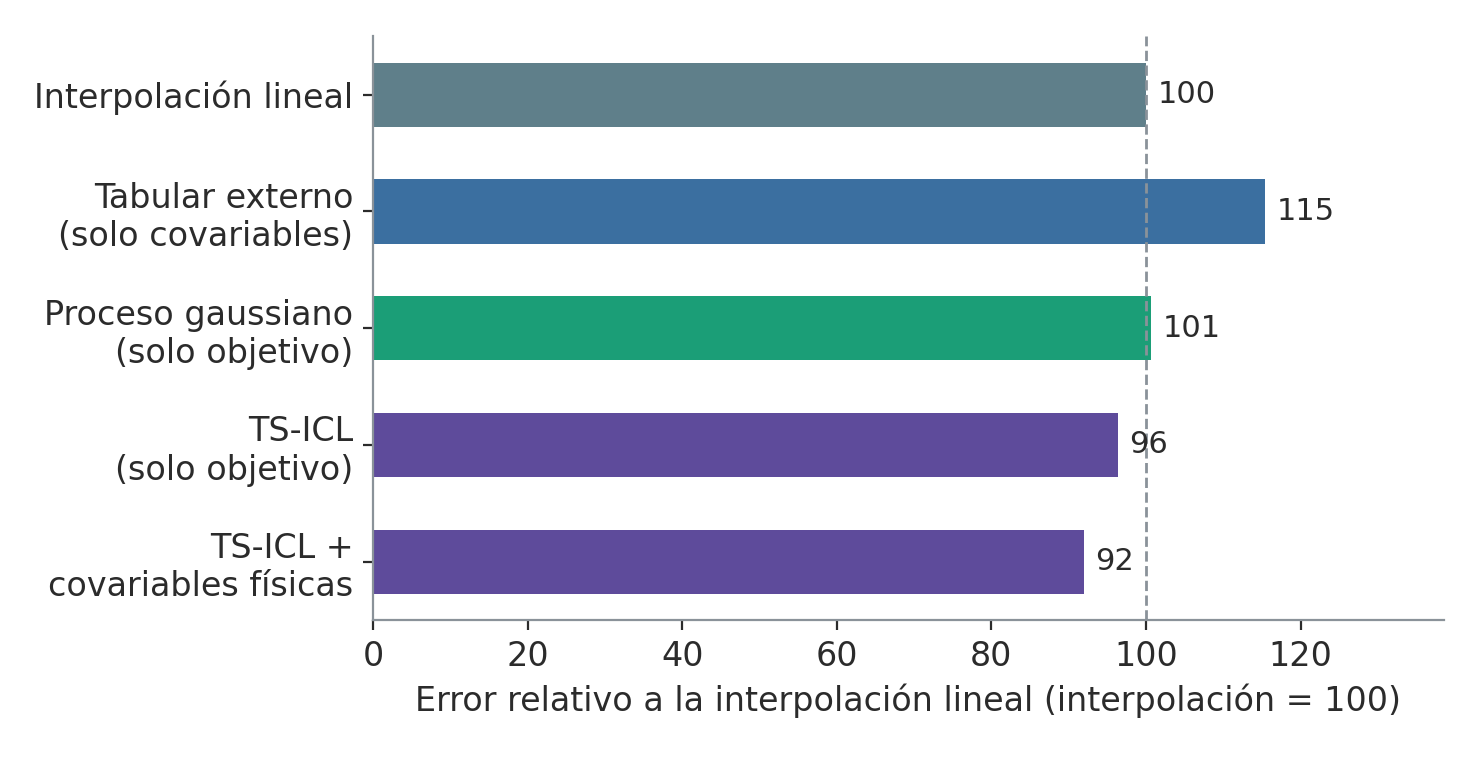
\includegraphics[width=0.56\textwidth]{figures/fig_d_oxygen_pooled_comparison.png}
  \end{center}
  \vskip2pt
  {\footnotesize\color{ink}
  \begin{itemize}\setlength\itemsep{0.05cm}
    \item Interpolación vuelve a ser una referencia fuerte.
    \item El tabular externo (solo covariables) vuelve a quedar por debajo de la
      interpolación --- igual que en clorofila.
    \item El mejor brazo es TS-ICL con el \textbf{paquete físico}: temperatura
      superficial del mar, viento/surgencia, radiación solar y corriente/transporte,
      combinados como canales de covariables.
  \end{itemize}}
\end{frame}

% ───────────────────────── DIAPOSITIVA 21 ─────────────────────────
\begin{frame}[t]{Caso oxígeno: las colas de la distribución}
  \vskip2pt
  \begin{center}
    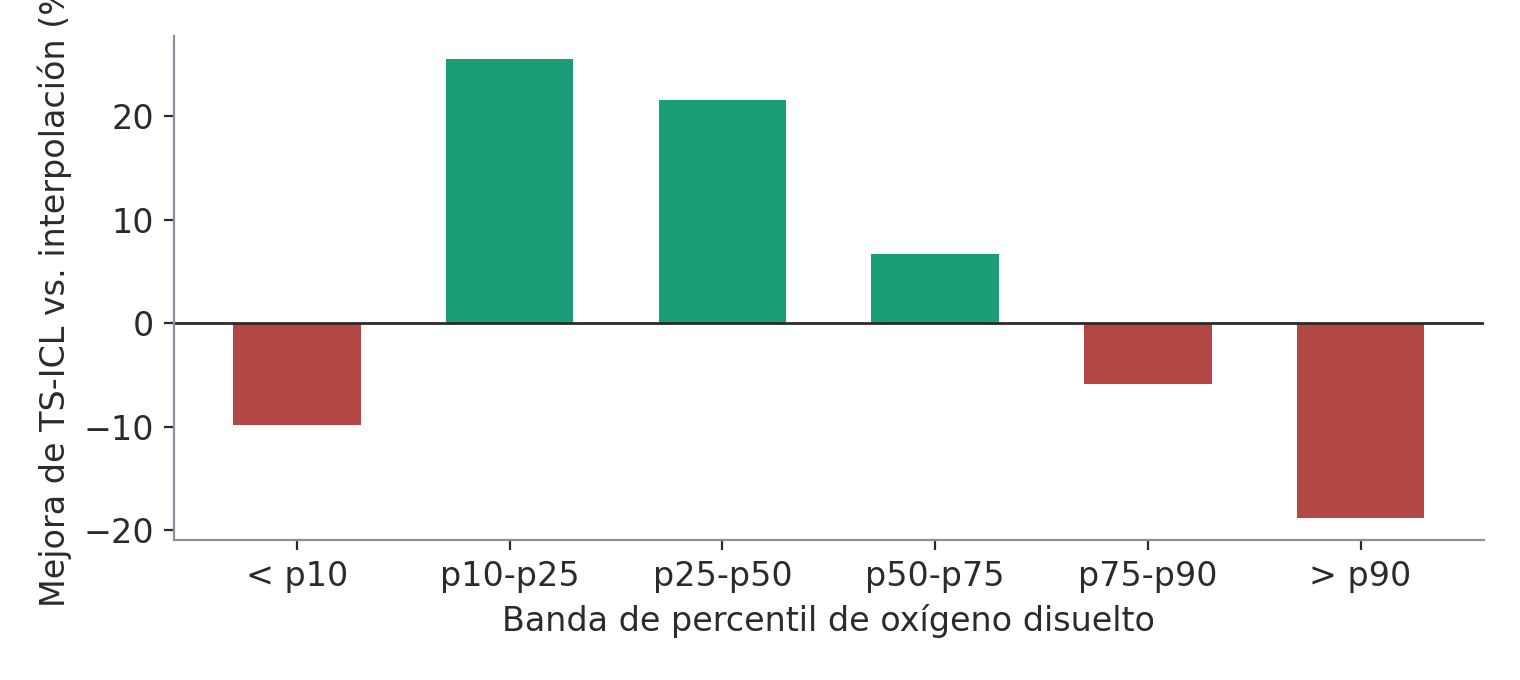
\includegraphics[width=0.58\textwidth]{figures/fig_e_oxygen_tail_comparison.png}
  \end{center}
  \vskip2pt
  {\footnotesize\color{ink}p10 y p90 aquí son \textbf{bandas empíricas de validación}
   (percentiles de la distribución de oxígeno observado), no umbrales ecológicos de
   hipoxia u otro criterio biológico.}
  \vskip0.1cm
  \caution{\centering La ganancia de TS-ICL se concentra en el rango medio. En ambos
   extremos (oxígeno muy bajo o muy alto) queda \textbf{peor} que la interpolación simple.}
\end{frame}

% ───────────────────────── DIAPOSITIVA 22 ─────────────────────────
\begin{frame}[t]{Covariables: alineadas versus placebo}
  \vskip4pt
  \begin{columns}[T]
    \begin{column}{0.44\textwidth}
      \vskip0.05cm
      {\scriptsize Una covariable cuenta como información reconstructiva útil solo si
       la versión alineada en el tiempo supera a versiones deliberadamente rotas:}
      \vskip0.1cm
      \cmpbox{accent}{\linewidth}{\scriptsize
        \textcolor{cgreen}{\textbf{alineada (real)}}\\[2pt]
        \textcolor{cred}{rezago incorrecto}\\[2pt]
        \textcolor{cred}{orden temporal rebarajado dentro de la estación del año}\\[2pt]
        \textcolor{cred}{año desplazado}\\[2pt]
        \textcolor{cred}{permutada}}
      \vskip0.1cm
      {\scriptsize\color{ink}Si la alineada no supera a las cuatro rotas, no hay
       información reconstructiva específica en el tiempo.}
    \end{column}
    \begin{column}{0.52\textwidth}
      \vskip0.02cm
      {\footnotesize\textbf{Clorofila}
      \begin{itemize}\setlength\itemsep{0.05cm}
        \item Viento / surgencia: señal alineada robusta.
        \item Temperatura superficial y corriente/transporte: no se estableció la misma
          evidencia.
      \end{itemize}}
      \vskip0.08cm
      {\footnotesize\textbf{Oxígeno}
      \begin{itemize}\setlength\itemsep{0.05cm}
        \item Corriente/transporte: informativa en aislamiento.
        \item Sin aporte adicional resuelto dentro del paquete físico completo (posible
          redundancia).
      \end{itemize}}
      \vskip0.08cm
      \takeaway{\footnotesize Información compartida en el tiempo --- \textbf{no}
       causalidad física.}
    \end{column}
  \end{columns}
\end{frame}

% ───────────────────────── DIAPOSITIVA 23 ─────────────────────────
\begin{frame}[t]{Límites y precauciones}
  \vskip10pt
  \begin{columns}[T]
    \begin{column}{0.49\textwidth}
      {\small\bfseries\color{accent}Límites de la validación}
      \vskip0.16cm
      {\footnotesize
      \begin{itemize}\setlength\itemsep{0.20cm}
        \item Un gap real \textbf{no tiene verdad conocida}: su reconstrucción es un
          candidato, no evidencia.
        \item Gaps muy largos (meses) quedan fuera de lo validado.
        \item Los eventos extremos son, en todos los casos, el régimen más difícil.
      \end{itemize}}
    \end{column}
    \begin{column}{0.49\textwidth}
      {\small\bfseries\color{accent}Límites físicos y de alcance}
      \vskip0.16cm
      {\footnotesize
      \begin{itemize}\setlength\itemsep{0.20cm}
        \item Los productos externos son más gruesos que la escala del sensor local.
        \item La evidencia de covariables es correlacional, no causal.
        \item La validación es de una sola estación; no está probado que transfiera a
          otra boya sin repetir el proceso.
      \end{itemize}}
    \end{column}
  \end{columns}
  \vskip0.30cm
  \takeaway{\centering{\bfseries\color{accent}Validar contra una línea de base fuerte,
   preservar el contexto físico, y revisar dónde falla el método, no solo el promedio.}}
\end{frame}

% ───────────────────────── DIAPOSITIVA 24 ─────────────────────────
\begin{frame}[t]{Conclusión operativa}
  \vskip8pt
  {\small
  \begin{enumerate}\setlength\itemsep{0.20cm}
    \item Comparar siempre primero contra la interpolación.
    \item Validar con gaps artificiales, de varias longitudes y estaciones del año.
    \item Comparar varios métodos usando el mismo protocolo.
    \item Preferir un método que, además de preciso, sea \textbf{operable} por el equipo.
    \item Usar la incertidumbre cuando esté disponible, no solo el valor puntual.
    \item Diagnosticar dónde falla el método (eventos, colas), no solo el error promedio.
  \end{enumerate}}
  \vskip0.3cm
  \takeaway{El producto principal de este proyecto \textbf{no es un modelo ganador}. Es un
   \textbf{flujo de validación reutilizable} para decidir, con evidencia, cómo reconstruir
   cualquier serie ambiental interrumpida.}
\end{frame}

% ═══════════════ BLOQUE E --- CAPACIDADES Y ADAPTACIÓN ═══════════════

% ───────────────────────── DIAPOSITIVA 25 ─────────────────────────
\begin{frame}[t]{Qué información usa cada método}
  \vskip6pt
  \begin{center}\scriptsize
  \renewcommand{\arraystretch}{1.15}
  \setlength{\tabcolsep}{3.2pt}
  \begin{tabular}{@{}l c c c c c c c@{}}
    \toprule
    Método & Historial & Cova- & Requiere & Ajuste & Salida & Evaluado & \\
     & del objetivo & riables & borde post. & local & prob. & en gap abierto & \\
    \midrule
    Persistencia            & \yes & \no  & \no  & \no  & \no  & \no & \\
    Climatología             & \yes\,(hist.) & \no  & \no  & \no  & \no  & \no & \\
    Interpolación lineal     & \yes\,(bordes) & \no  & \yes & \no  & \no  & \no & \\
    Proceso gaussiano        & \yes & \no  & \no  & \yes & \yes & \no & \\
    Tabular externo          & \no  & \yes & \no  & \yes & \no  & \no & \\
    Residuo de borde         & \yes\,(bordes) & \weak\,(opc.) & \yes & \yes & \no  & \no & \\
    TS-ICL solo-objetivo     & \yes & \no  & \no  & \no\,(zero-shot) & \yes & \no & \\
    TS-ICL + covariables     & \yes & \yes & \no  & \no\,(zero-shot) & \yes & \no & \\
    \bottomrule
  \end{tabular}
  \end{center}
  \vskip0.12cm
  {\scriptsize\color{ink}``Requiere borde posterior'' es una propiedad técnica del
   método; ``evaluado en gap abierto'' es una afirmación de validación aparte ---
   ningún método aquí, incluidos GP y TS-ICL, fue evaluado en un escenario de gap
   abierto (sin contexto futuro): el protocolo de validación de este proyecto siempre
   opera sobre gaps cerrados y retrospectivos. Verificado contra el código, no supuesto.}
\end{frame}

% ───────────────────────── DIAPOSITIVA 26 ─────────────────────────
\begin{frame}[t]{Adaptar esto a otra variable o estación}
  \vskip4pt
  {\small
  \begin{enumerate}\setlength\itemsep{0.055cm}
    \item Definir el objetivo diario: variable, unidad, regla de agregación, control de
      calidad.
    \item Auditar gaps reales.
    \item Identificar qué historial del objetivo y qué covariables hay disponibles.
    \item Construir gaps artificiales cubriendo varias longitudes y estaciones del año.
    \item Correr líneas de base fuertes primero.
    \item Comparar métodos con historial del objetivo, externos, y TS-ICL bajo el mismo
      protocolo.
    \item Revisar eventos, colas de la distribución, e incertidumbre --- no solo el
      promedio.
    \item Aplicar el método elegido a los gaps reales.
    \item Exportar procedencia y advertencias junto con cada reconstrucción.
  \end{enumerate}}
  \vskip0.05cm
  \takeaway{\footnotesize TS-ICL se evalúa solo-objetivo desde el principio; las
   covariables son opcionales y se agregan probándolas, no asumiéndolas.}
\end{frame}

% ───────────────────────── DIAPOSITIVA 27: CIERRE ─────────────────────────
% Nota para el orador (no se muestra en la diapositiva): después de cerrar
% las diapositivas mostraré una demo local del flujo de reconstrucción.
% El repositorio y las instrucciones de instalación se mencionan solo de
% forma oral en ese momento, no en esta diapositiva.
\begin{frame}[t]{Mensaje final}
  \vskip8pt
  {\small
  \begin{itemize}\setlength\itemsep{0.26cm}
    \item Los gaps reales no validan por sí mismos una reconstrucción.
    \item La comparación debe hacerse con gaps artificiales, estratificada por
      longitud y régimen.
    \item La interpolación es una referencia fuerte.
    \item TS-ICL es útil porque permite reconstrucción zero-shot, con covariables
      opcionales y con incertidumbre.
    \item Los eventos extremos siguen siendo el régimen crítico.
  \end{itemize}}
  \vskip0.5cm
  \begin{center}
  {\Large\color{accent}\bfseries Preguntas}
  \end{center}
\end{frame}

\end{document}
